\documentclass[a4paper,12pt,oneside]{article}


\usepackage[english]{babel}
\usepackage{caption}
\usepackage[T1]{fontenc}
\usepackage[utf8]{inputenc}
\usepackage{fancyhdr}
\usepackage{lscape}

\usepackage{lmodern}

\usepackage[normalem]{ulem}
\usepackage[left=3cm,right=2cm,top=1.5cm,bottom=1cm,
includeheadfoot,headsep=1cm,
footskip=1cm,headheight=14.599pt]{geometry}

\usepackage[backend=biber, style=apa]{biblatex}
\usepackage{graphicx} 
\usepackage{epstopdf}

\usepackage{threeparttable} % For adding notes below the table
\usepackage{tabularx}
\usepackage{longtable}
\usepackage{booktabs}
\usepackage{multirow}

\usepackage{subcaption}

\usepackage{csquotes}


\usepackage{amsmath}
\usepackage{amsthm}
\usepackage{amsfonts}

\usepackage{setspace}
\onehalfspacing

\usepackage{tikz}

\usepackage{adjustbox}
\usepackage{float}

\usepackage{tcolorbox}
\tcbset{colback=white,colframe=orange,
        fonttitle=\bfseries}

\usepackage[colorlinks,pdfpagelabels,pdfstartview=FitH,
bookmarksopen=true,bookmarksnumbered=true,linkcolor=black,
plainpages=false,hypertexnames=false,citecolor=black]{hyperref}


\usepackage{listings}
\usepackage{xcolor}

\usepackage[skip=12pt, indent=0pt, parfill=50pt]{parskip}

\definecolor{codegreen}{rgb}{0,0.5,0} % Slightly darker green for comments
\definecolor{codegray}{rgb}{0.4,0.4,0.4} % Darker gray for line numbers
\definecolor{codepurple}{rgb}{0.5,0,0.5} % A more subdued purple for strings
\definecolor{backcolour}{rgb}{0.98,0.98,0.98} % A lighter background for better contrast

\lstdefinestyle{codeStyle}{
    backgroundcolor=\color{backcolour},   
    commentstyle=\color{codegreen},
    keywordstyle=\color{magenta},
    numberstyle=\tiny\color{codegray},
    stringstyle=\color{codepurple},
    basicstyle=\ttfamily\footnotesize,
    breakatwhitespace=false,         
    breaklines=true,                 
    captionpos=b,                    
    keepspaces=true,                 
    numbers=left,                    
    numbersep=5pt,                  
    showspaces=false,                
    showstringspaces=false,
    showtabs=false,                  
    tabsize=2
}
\lstset{style=codeStyle}

\addbibresource{bib/literature.bib}
\addbibresource{bib/sites.bib}


\renewcommand{\thesubfigure}{\arabic{subfigure}}

%%%%%%%%%%%%%%%%%%%%%%%%%%%%%%%%%%%%%%%%%%%%%
%% DOCUMENT                                %%
%%%%%%%%%%%%%%%%%%%%%%%%%%%%%%%%%%%%%%%%%%%%%
\begin{document}
    \pagenumbering{gobble}
    

    \pagestyle{empty}
    \begin{titlepage}
    \begin{figure}[!ht]
        % \flushleft
            
\includegraphics[width=0.26\textwidth]{sources/logo_TH-Koeln_CMYK_22pt.eps}
    \end{figure}

    \begin{center}
      \Large
      Cologne University of Applied Sciences\\
      Faculty of Computer Science and Engineering Science\\
      \vspace{0.5cm}
      \hrule\par\rule{0pt}{2cm}
      \LARGE
      \textsc{M A S T E R  T H E S I S}\\
      \vspace{1cm}
      \huge
      Texture Asset generation through Transformer Models\\
      \vspace{1.5cm}
      \large
      Cologne University of Applied Sciences\\
      Campus Gummersbach\\
      Master Digital Sciences\\ 
      \vspace{1.0cm}
      written by:\\
      \textsc{Dennis Goßler}\\
      11140150\\
      \vspace{1.5cm}
      \begin{tabular}{ll}
          \textbf{First examiner:} & Prof. Dr. Olaf Mersmann \\
          \textbf{Second examiner:} & Prof. Dr. Boris Naujoks \\
      \end{tabular}
    
    \end{center}    
    \end{titlepage}
    
    \newpage
    
    
    \begin{abstract}
    TODO
    \end{abstract}
    
    \newpage
    

    \tableofcontents
    
    \newpage
    \pagestyle{fancy}
    
    
    \addcontentsline{toc}{section}{List of Figures}
    \listoffigures
    \newpage
    
    \addcontentsline{toc}{section}{List of tables}
    \listoftables
    \newpage
    
  
    \pagenumbering{arabic}
    
    \section{Introduction}\label{introduction}  
    
In this thesis, we will investigate the use of a traditional Transformer model to generate texture assets to use as floor texture in e.g. in video games. Transformers are usually used to ... . But in this thesis, the focus is to use them to generate the next Pixel in a texture. Multiple different datasets of textures will be used from the internet to train the model. The final developed models will be trained on a GPU cluster in Berlin. The models will be evaluated on a set of metrics and the results will be compared to other models.

\subsection{Related work}
    
\subsection{Data}
    
This section describes the methods used for gathering, cleaning, and analyzing data in a research thesis on textures. Essential for training a machine learning model, the data is carefully collected from various sources, cleaned to maintain uniformity, and examined for patterns, with a focus on color distribution.


\subsubsection{Data Retrieval}
On the internet, a wide variety of textures can be found, but not all of them are suitable for this task. The textures should be seamless, devoid of shadows, and free from any objects. Textures of floors, such as carpets, tiles, wood, concrete, and more, were utilized. Two approaches were employed to acquire the data for this thesis.

\begin{itemize}
    \item Web Data Collection

    The data for this project was obtained from various online sources. Numerous free texture providers, such as textures.com, texturehaven.com, and others, were utilized for data acquisition. Due to the limitation of downloading one texture at a time from most websites, a series of scripts were developed to compile a list of suitable textures and automate the downloading process. These scripts were created using UiPath and Python.
    
    \item Video Game Textures
    
    The second approach involved using textures from video games. The advantage of this approach is that these textures are already seamless and often of high quality and quantity. However, a drawback is that these textures can be very repetitive. To obtain these textures, downward-facing recordings of the game were made, and the textures were extracted from the video. The major challenge with this approach is the need to disable shadows and all UI elements (HUD elements) in the game, which is not always possible.
\end{itemize}

\subsubsection{Data Cleaning}

    To ensure that the data is consistent and free from elements that could corrupt the model, various cleaning steps were applied. For example, all images containing 3D objects were removed, especially those gathered from video games. During the recording of the floor, unwanted debris or pieces of wood were often present, and all extracted frames were manually checked.

    In the case of web-gathered textures, there were different folder structures, and it was necessary to standardize them across all data folders. Additionally, some of them had associated files that were irrelevant to this use case and needed to be discarded.

    All the images were in high-definition (HD) quality, with a height of approximately 1024 pixels.


    \begin{table}[h]
        \centering
        \begin{tabular}{|c|c|c|}
            \hline
            Dataset & Size & Number of Images \\
            \hline
            FreePBR & 452.0 MB & 263 \\
            Polyhaven & 298.0 MB & 439 \\
            Poliigon & 70.4 MB & 49 \\
            Minecraft-Textures &  636.0 MB & 493 \\
            CsGoFloor-Textures & 18.3 GB & 44540 \\
            \hline
            Combined & 20.2 GB & 45784 \\
            \hline
        \end{tabular}
        \caption{Datasets collected for this thesis}
        \label{tab:datasets}
    \end{table}

    \subsubsection{Patterns in the data}
    
    To examine whether the dataset encompasses a broad spectrum of colors, multiple plots are created. These plots illustrate the color distribution within the datasets, providing insights into the diversity of colors present. Prior to plotting, a comprehensive pixel count across all images is conducted. For instance, if an image features 10 pixels of the color $(255, 0, 0)$, this count is added to a dictionary. Should the subsequent image in the dataset contain 5 pixels of the same color, these are also incorporated into the dictionary, cumulating a total of 15 for that specific color. This process is repeated for each color encountered, aggregating the counts to yield the overall color frequency within the dataset.

\begin{lstlisting}[language=Python]
  color_counts = {} 
  for i, (data, _) in enumerate(dataset):
      # data is a tensor of shape (3, height, width) 
      pixel_rgb_array = (data.view(3, -1).t() * 255).to(torch.int32)
      
      for pixel_color in map(tuple, pixel_rgb_array):
          if color in color_counts:
              color_counts[pixel_color] += 1
          else:
              color_counts[pixel_color] = 1
\end{lstlisting}

    After analyzing the dataset through this method, visual representations of the color distributions were produced using Python and Matplotlib. These plots provide a three-dimensional view of the RGB color space, where the X, Y, and Z axes correspond to the Red, Green, and Blue color values, respectively, each ranging from 0 to 255. 

    \[
    \text{size} = \log(\text{count of color}) \times 20
    \]

    The size of each plotted point is calculated based on the logarithm of the color count, scaled by a factor of 20.
    
    

    \begin{figure}[htbp]
        \centering
        
        \begin{subfigure}{.33\textwidth}
          \centering
          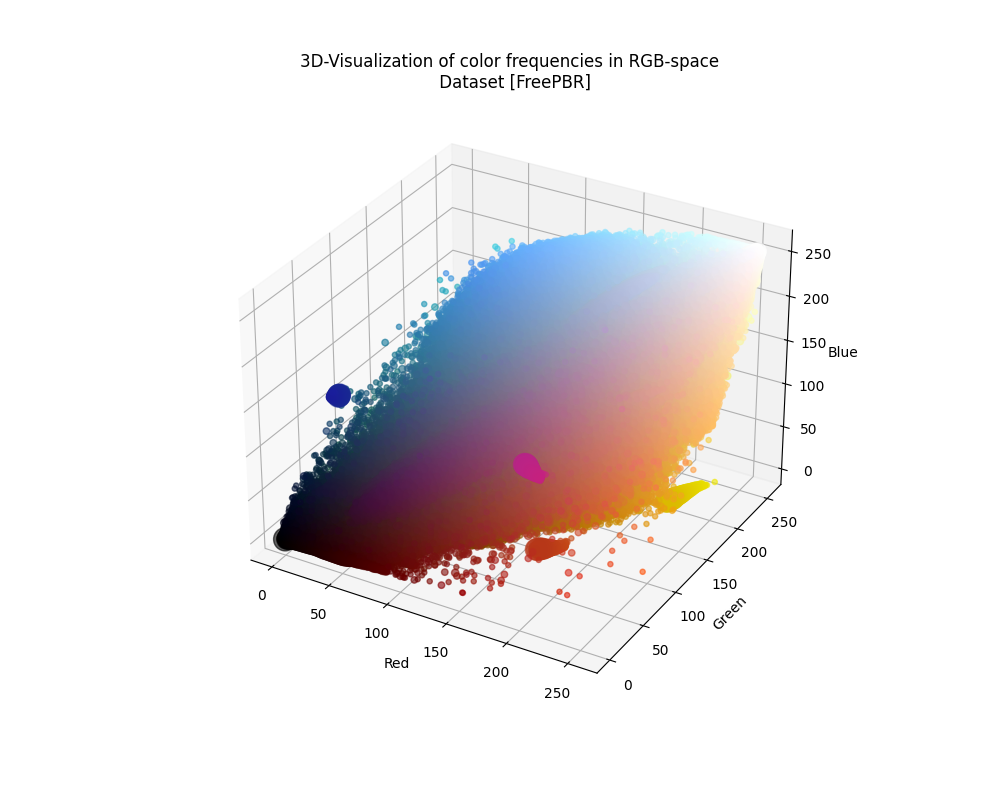
\includegraphics[width=\linewidth]{../code/dataAnalysis/output/FreePBR.png}
          \caption{FreePBR}
          \label{fig:dataset-FreePBR}
        \end{subfigure}%
        \hfill
        \begin{subfigure}{.33\textwidth}
          \centering
          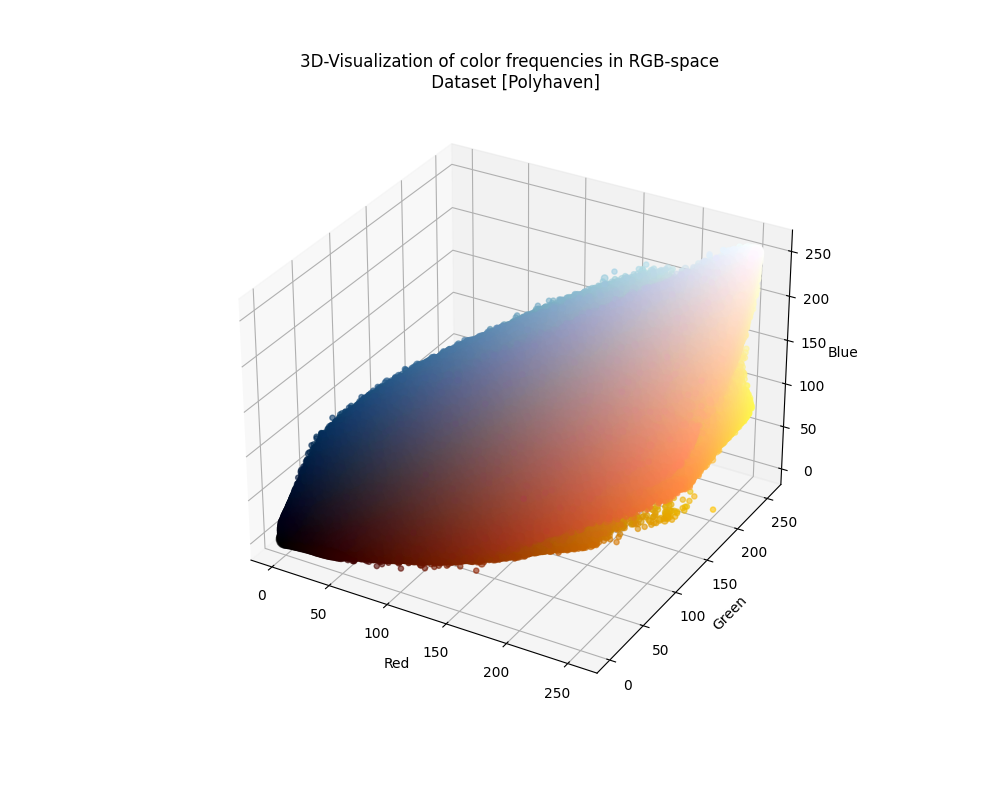
\includegraphics[width=\linewidth]{../code/dataAnalysis/output/Polyhaven.png}
          \caption{Polyhaven}
          \label{fig:dataset-Polyhaven}
        \end{subfigure}%
        \hfill
        \begin{subfigure}{.33\textwidth}
          \centering
          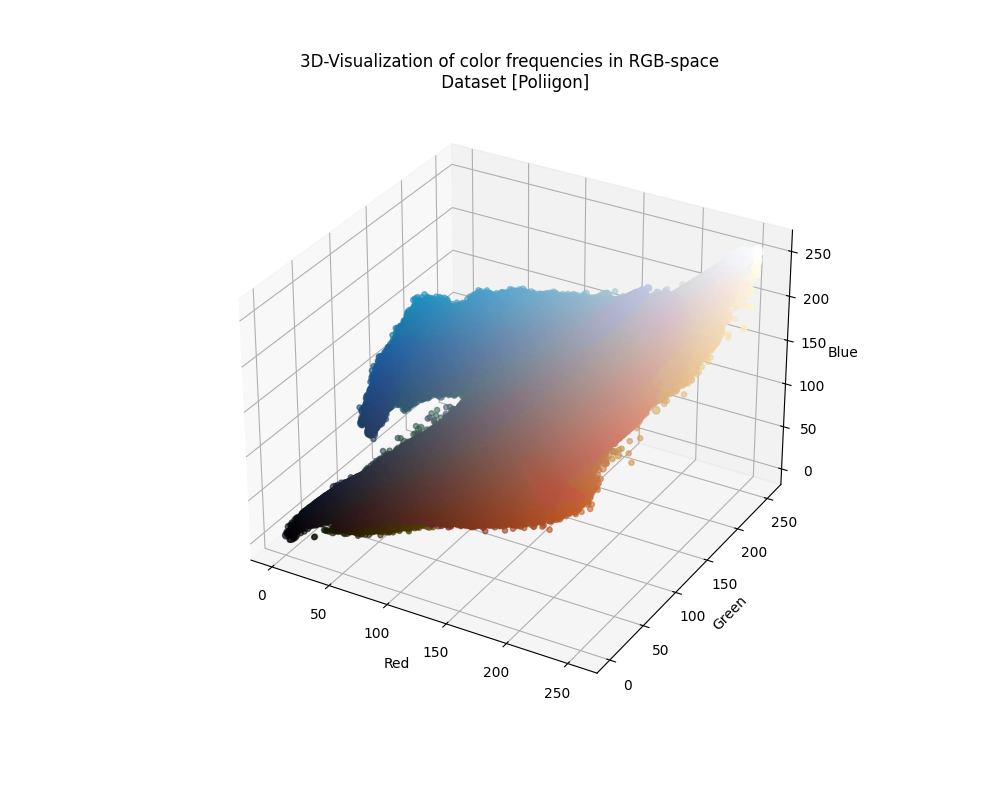
\includegraphics[width=\linewidth]{../code/dataAnalysis/output/Poliigon.png}
          \caption{Poliigon}
          \label{fig:dataset-Poliigon}
        \end{subfigure}
        
        \vspace{1cm} % Vertikaler Abstand zwischen den Reihen
        
        \begin{subfigure}{.33\textwidth}
          \centering
          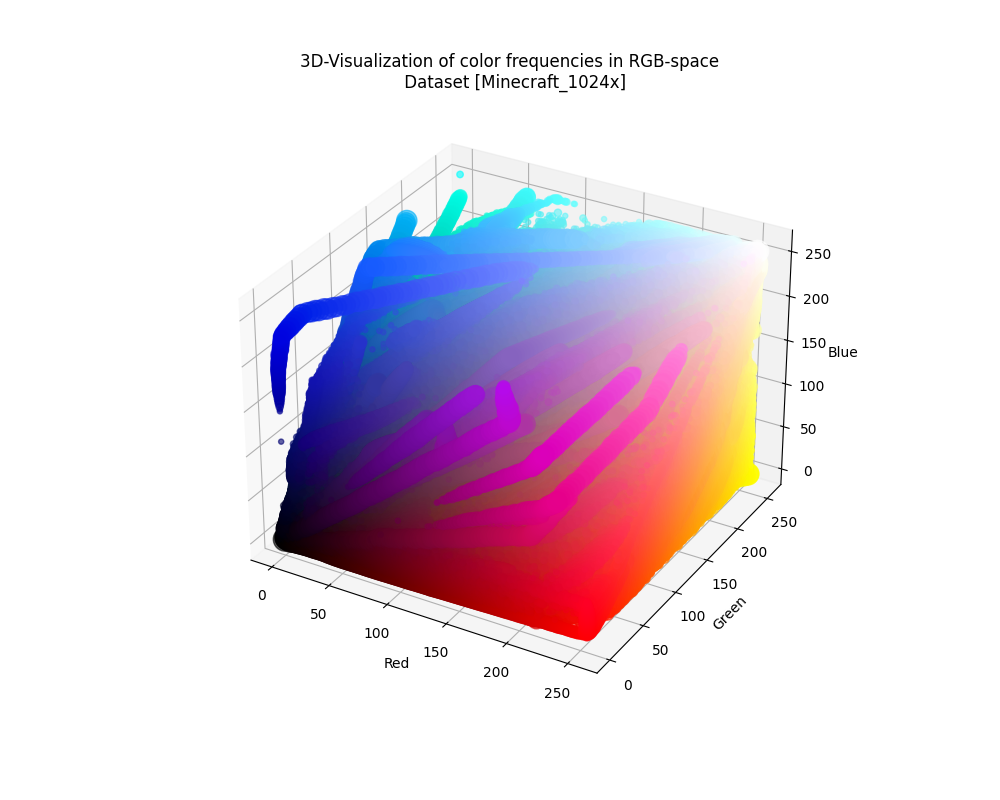
\includegraphics[width=\linewidth]{../code/dataAnalysis/output/Minecraft_1024x.png}
          \caption{Minecraft-Textures}
          \label{fig:dataset-Minecraft-Textures}
        \end{subfigure}%
        \hfill
        \begin{subfigure}{.33\textwidth}
          \centering
          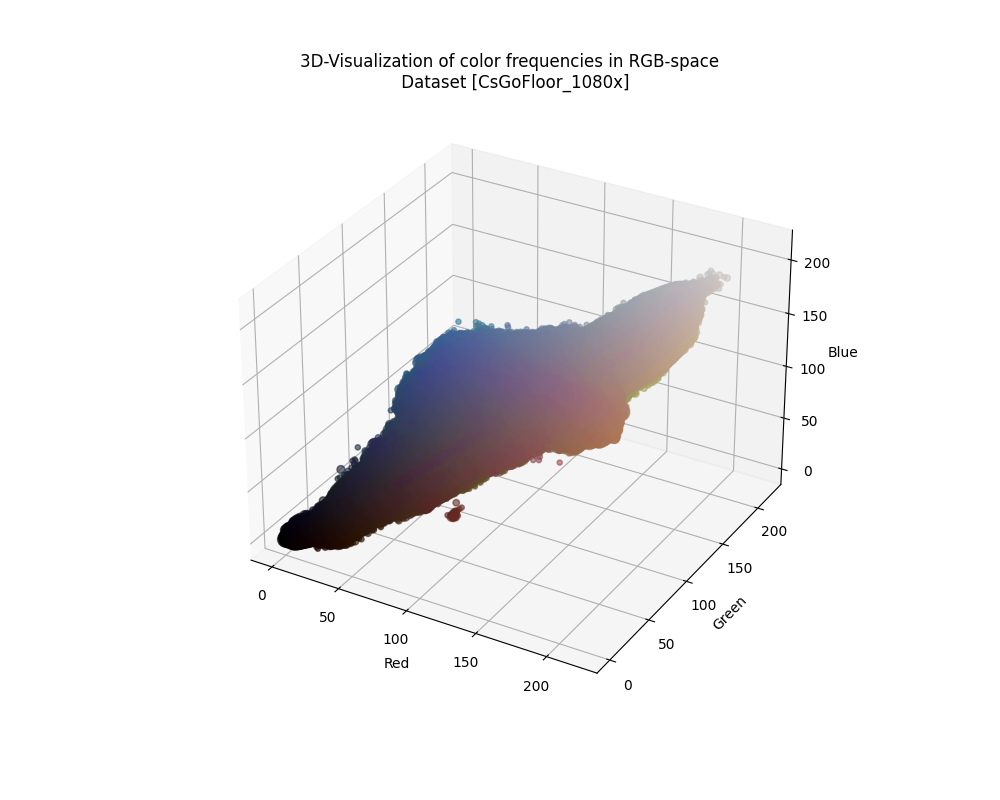
\includegraphics[width=\linewidth]{../code/dataAnalysis/output/CsGoFloor_1080x.png}
          \caption{CsGoFloor-Textures}
          \label{fig:dataset-CsGoFloor-Textures}
        \end{subfigure}%
        \hfill
        \begin{subfigure}{.33\textwidth}
            \centering
            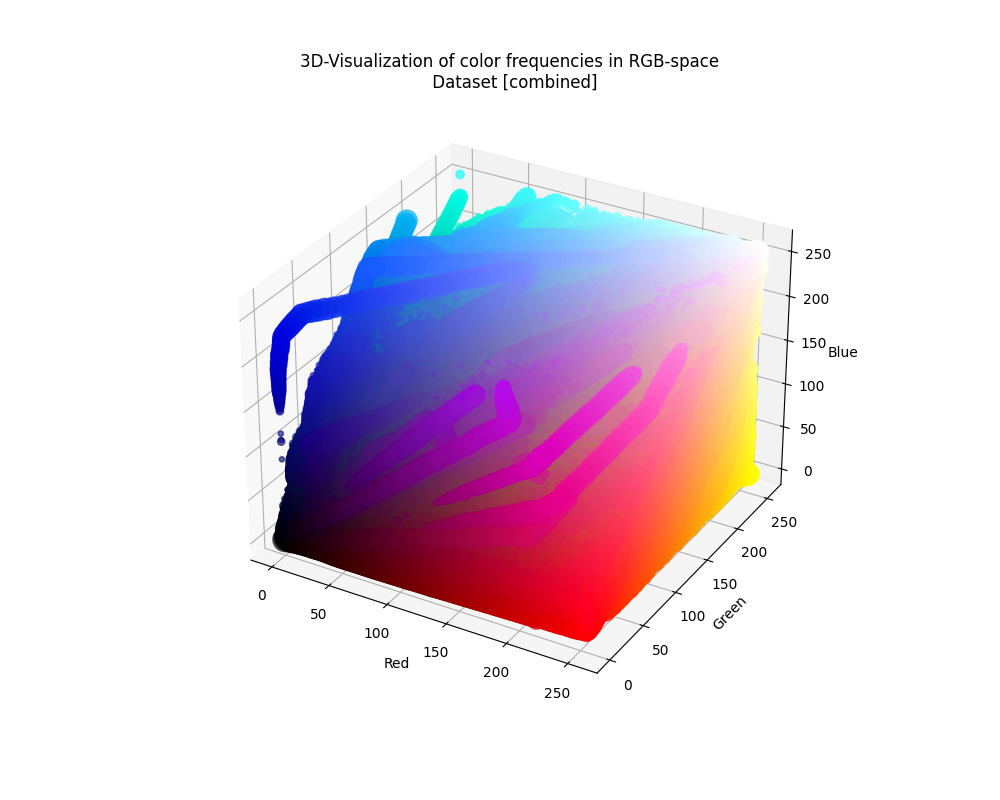
\includegraphics[width=\linewidth]{../code/dataAnalysis/output/combined.png}
            \caption{Combined}
            \label{fig:dataset-Combined}
        \end{subfigure}%
        \hfill
    \end{figure}

    In the figure above, the color distributions of the individual datasets are shown. The first five subfigures represent the color distributions of the individual datasets, while the last subfigure (\ref{fig:dataset-Combined}) shows the combined color distribution of all datasets. The color distributions of the individual datasets are quite similar, except for the Minecraft-Textures dataset, which is way more colorful than the others. The combined figure is a combination of all the individual datasets, and it is evident that the color distribution is quite diverse. This is a positive sign, as it indicates that the dataset is not focused on only a specific color spectrum.

    \subsubsection{Data Synchronization}

    In the thesis, a manual data synchronization routine is established to maintain data consistency between the supercomputer located in Berlin and the local workstation.

\subsection{Training process}
    (gpu cluster göthingen, my GPU, ...)

\subsection{Models}
    (LLMs, basic idea, roll model, spiral model) 
    \newpage

    \section{Experiment}
    
    \subsection{The Foundation of the Models}

    To build the models, a set of Python libraries is utilized, mainly PyTorch, NumPy, TensorBoard, and Einops. PyTorch serves as the core tool for constructing and training the models.
    
    The models discussed in this thesis are based on a Python script by A. Karpathy named NanoGPT \autocite{nanoGPTkarpathy2023}. This script demonstrates a straightforward and accessible GPT implementation. 
    
    \subsubsection{Data Handling}
    
    For data management, a script named dataSetCombiner is developed to load and return a combined dataset from specified image folders with optional transformations. The function combines the 33 different sources from multiple directories into a single dataset, also offering the option to apply various image transformations such as cropping, flipping, gray scaling, and color jitter.
    
    It allows for the selection between 512x512 and 1024x1024 pixel datasets, depending on the use case. Parameters can be adjusted to tailor the dataset to specific needs, such as image size, the particular dataset to load, and the option to include multiple instances of the dataset. Furthermore, it can randomly flip images vertically or horizontally to augment the dataset, thereby preventing overfitting and improving model generalization. It also supports color jittering, allowing for random adjustments in image brightness, contrast, saturation, and hue, which introduces further variability into the dataset when needed. Additionally, an option to convert images to grayscale is available.
    

\begin{figure}[H]
\centering
\begin{lstlisting}[language=Python]
    def getDataSet(path, dataset_name, size_x, size_y, repeatData=1, random_vertical_flip=False, random_horizontal_flip=False, crop_type='random', grayscale=False, color_jitter=False, jitter_brightness=0, jitter_contrast=0, jitter_saturation=0, jitter_hue=0):
\end{lstlisting}
\caption{Python function declaration: getDataSet}
\label{fig:getDataSet}
\end{figure}


    \subsubsection{Monitoring Training Progress}
    
    The training process is monitored using TensorBoard, a tool that helps visualize different aspects of training. In this thesis, TensorBoard is particularly useful for tracking training and validation loss through plots. It also allows for the viewing of the input images and the outputs generated by the models.    
    
\newpage


\subsection{Column Image Transformer}
    
    The Column Image Transformer is a transformer-based model that processes input data in a columnar format as examined in detail see \autoref{sec:IntroColumnModel}.
    
    \subsubsection{Get Data as Columns}

    The data is loaded as a DataLoader object, which is then iterated over to obtain the data in (Batch, Color, Height, Width) format. The data is then reshaped into a columnar format, resulting in a tensor of shape (Batch, Height, Color). This reshaping is achieved by indexing the data tensor as follows:

\begin{figure}[H]
\centering
\begin{lstlisting}[language=Python]

# data: (Batch, Color, Height, Width)
def get_batch(data):

    x = data[:, :BLOCK_SIZE, :BATCH_SIZE]
    y = data[:, 1:BLOCK_SIZE+1, :BATCH_SIZE]

    x = rearrange(x, 'c h b -> b h c')
    y = rearrange(y, 'c h b -> b h c')

    return x, y
\end{lstlisting}
\caption{Python function to convert data into a columnar format}
\label{fig:get_batch_CIT}
\end{figure}

    The resulting tensor \(x\) is the input to the model, and the tensor \(y\) is the target output. The \(y\) tensor is shifted by one position to the right so that the model can learn to predict the next column based on the previous columns.

    \subsubsection{Pixel Embedding}

    The input part of the data \(x\) is embedded into a higher-dimensional space using pixel embedding layers. This MLP is a straightforward linear layer that maps the input data to a higher-dimensional space, transitioning from 3 color channels to \(N_{\text{EMBD}}\). This layer consists of a linear transformation followed by a ReLU activation function and is succeeded by a dropout layer.

    Through testing and experimentation, it was discovered that the optimal configuration for the pixel embedding layer involves a specific sequence of dimensionality increases. The most effective pathway identified begins by scaling the dimensionality of the input from the original image channels \(C\) to one-fifth of \(N_{\text{EMBD}}\) (\(\frac{1}{5}N_{\text{EMBD}}\)), then increasing it to one-half of \(N_{\text{EMBD}}\) (\(\frac{1}{2}N_{\text{EMBD}}\)) until reaching \(N_{\text{EMBD}}\). The pixel embedding layer is followed by a dropout layer with a dropout rate of 0.2.

    It is crucial to highlight the importance of excluding a layer normalization (layernorm) layer in the initial few layers of the model. Incorporating layernorm early on results in outputs that are predominantly black and white. This phenomenon occurs because the color channels \(C\), which are comprised of Red, Green, and Blue, are normalized by the layernorm layer to exhibit uniform values across these channels. As a consequence, this normalization process hinders the model's ability to learn the distinct colors of the pixels, relegating it to only wrong grayscale variations.

    \subsubsection{Positional Embedding}

    \subsubsection{Classification or Regression}

    \subsubsection{Discriminator}

\newpage


\subsection{Spiral Image Transformer}
    (explanation, Data to Spiral form, positional embedding, )

    As explained in the previous section (see Section \ref{sec:IntroSpiralModel}), the spiral model is a transformer-based model that employs a spiral architecture to process input data. 

    \subsubsection{Spiral}

    To convert the 3-dimensional data (color channels, image height, image width) into a spiral form, the data must be unrolled into one dimension, resulting in an output format of (color channels, spiral length). Consequently, the data width and the height dimensions must be squeezed into a single dimension. This new form can then be utilized similarly to the data in the Column Image Transformer. As the data is flattened into a single dimension, it allows for an easy addition of positional embedding.

    \subsubsection{Spiral generation}

    The conversion of data into a spiral form needs to be highly efficient because the code block will execute for every image (batch) in the dataset. Therefore, a simple nested for loop is insufficient. In this example, fancy indexing is used to convert the data into a spiral form. Thus, the data tensor is indexed with a two-dimensional tensor containing the indices of the spiral form.

    At the start of the model training script, one indexing spiral is created to be used for all images in the dataset. The following code block illustrates the creation of the spiral index tensor.

\begin{figure}[H]
\centering
\begin{lstlisting}[language=Python]
def create_spiral(n): # n = width and height
    
    matrix = [[0] * n for _ in range(n)] # Initialize n x n matrix

    x, y = 0, 0
    # Direction vectors (right, down, left, up)
    dx = [0, 1, 0, -1]
    dy = [1, 0, -1, 0]
    direction = 0

    for i in range(n * n - 1, -1, -1):  # Start (35 for 6x6)
        matrix[x][y] = i
        nx = x + dx[direction]
        ny = y + dy[direction]

        # Change direction if the next position: out of bounds or filled
        if nx<0 or nx>=n or ny<0 or ny>=n or matrix[nx][ny]!=0:
            direction = (direction + 1) % 4  # Change direction
            nx = x + dx[direction]
            ny = y + dy[direction]

        x, y = nx, ny
    
    return torch.tensor(matrix)
\end{lstlisting}
\caption{Python function to create a spiral index tensor}
\label{fig:spiral_matrix}
\end{figure}

    The code above generates a square matrix of size n by n, then fills it with numbers in a spiral pattern, starting from the outer edge and spiraling inwards clockwise. Each cell of the matrix is assigned a unique number, beginning from the highest value in the top-left corner and decreasing by one with each step along the spiral path until reaching zero at the center or the end of the spiral. The spiral formation is achieved by moving right, then down, then left, then up, and repeating this sequence, adjusting direction whenever the next step would go out of bounds or into a cell that's already been filled.


    \subsection{Fancy Indexing into the Spiral form}

    The spiral index tensor is then used to index the data tensor, effectively converting it into a spiral form. The following image illustrates the process of converting a 7x7 image.
    
    
    \begin{figure}[H]
    \centering
    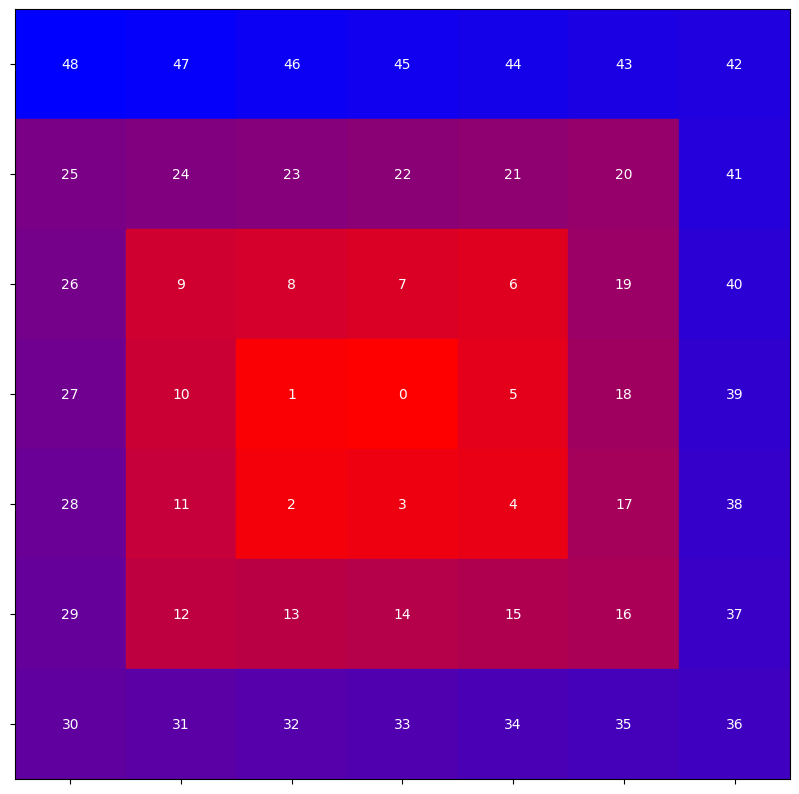
\includegraphics[width=0.6\textwidth]{../code/dataAnalysis/plots/exampleImgs/spiralShowcase1.png}
    \caption{Image representation}
    \label{fig:spiral_indexing_1}        
    \end{figure}

    \begin{figure}[H]
    \centering
    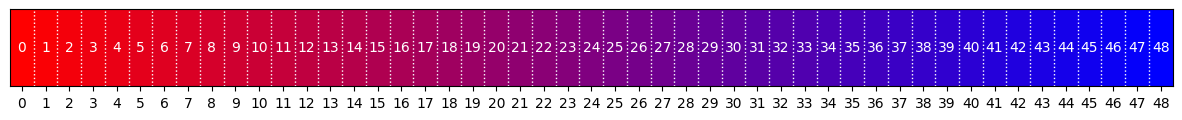
\includegraphics[width=1\textwidth]{../code/dataAnalysis/plots/exampleImgs/spiralShowcase0.png}
    \caption{7x7 Image flattened into a spiral form} 
    \label{fig:spiral_indexing_0}        
    \end{figure}

    As you can see in \autoref{fig:spiral_indexing_1}, the pixels of the image are labeled with their respective indices 0, \dots, 43. The image is then unrolled into a single dimension, as shown in \autoref{fig:spiral_indexing_0}. The centering pixel is the first element of the spiral, and the spiral continues counterclockwise from there. In the model script, the dimensions for width and height typically exceed 7, yet the underlying process remains unchanged.

\begin{figure}[H]
\centering
\begin{lstlisting}[language=Python]
  spiral_indices = torch.tensor(create_spiral(IMAGE_SIZE))

  # [...]
  # Batch_size, Color_channels, Height, Width
  B, C, H, W = data.shape

  spiral_data = torch.zeros_like(data.view(B, C, -1))

  spiral_data[:,:,spiral_indices.flatten()] = data.view(B, C, -1)

  # [...]
\end{lstlisting}
\caption{Fancy indexing to convert data into a spiral form}
\label{fig:spiral_indexing_code}
\end{figure}

    \subsubsection{Positional embedding}

\subsection{Problems}
    (layer norm(sigmoid vs clamp), color shift to gray (illustrations of average color), Text tokens vs imgs tokens)
    \newpage
    \subsection{Column Image Transformer}
    
    The Column Image Transformer (CIT) is the first transformer-based model approach in this thesis. It processes input data in a columnar format as examined in the previous section in more detail see \autoref{sec:IntroColumnModel}.


    \begin{figure}[H]
        \centering
        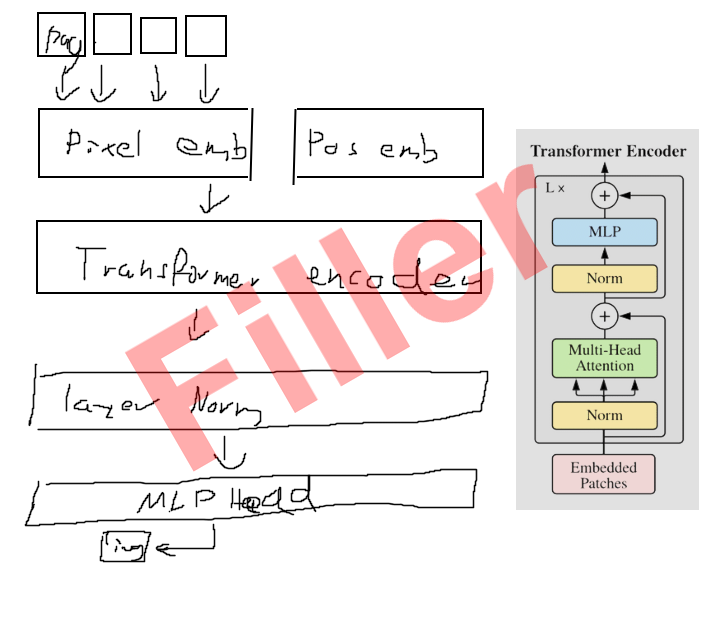
\includegraphics[width=0.8\textwidth]{imgs/CITModel.png}
        \caption{Column Image Transformer model structure}
        \label{fig:ColumnImageTransformer}
    \end{figure}

    The image above shows the steps carried out by the CIT model. The input data is reshaped into a columnar format, which is then embedded into a higher-dimensional space. The positional embedding layer adds positional context to the input data. The transformer layer processes the data, and the output is then transformed back into a columnar format. After going through a final layer normalization and another MLP that converts back from the embedded layer to 3 colors, the model is trained using a Mean Squared Error (MSE) loss function.

    \subsubsection{Get Data as Columns}

    The data is loaded into a DataLoader object as described in \autoref{sec:DataHandling} and iterated over to extract it as a 4-dimensional tensor (Batch, Color Channels, Height, Width). This data is reshaped into a columnar format, resulting in two tensors: the \(source\) and \(targets\), both with the shape (Batch, Height, Color Channels). The target tensor is shifted one pixel downwards to the prediction of subsequent pixels by the model. This reshaping and shifting method is commonly employed in transformer-style learning because it enables the model to process data more efficiently in terms of computational speed and resource utilization. The source tensor is then fed into the model, and its output is compared against the targets using the Mean Squared Error (MSE) loss function.

\begin{figure}[H]
\centering
\begin{lstlisting}[language=Python]
# data: (Batch, Color, Height, Width)
def get_batch(data):

    source = data[:, :BLOCK_SIZE, :BATCH_SIZE]
    targets = data[:, 1:BLOCK_SIZE+1, :BATCH_SIZE]

    source = rearrange(source, 'c h b -> b h c')
    targets = rearrange(targets, 'c h b -> b h c')

    return source, targets
\end{lstlisting}
\caption{Python function to convert data into a columnar format}
\label{fig:get_batch_CIT}
\end{figure}

    \subsubsection{Pixel Embedding}

    The \(source\) data is embedded into a higher-dimensional space using pixel embedding layers. This MLP is a straightforward linear layer that maps the input data to a higher-dimensional space, transitioning from \(3\) color channels to \(N_{\text{EMBD}}\). This layer consists of a linear transformation followed by a ReLU activation function and is succeeded by a dropout layer.

    Through testing and experimentation, it seems that the optimal configuration for the pixel embedding layer involves a sequence of dimensionality increases. The most effective pathway identified begins by scaling the dimensionality of the input from the original image channels \(C\) to one-fifth of \(N_{\text{EMBD}}\) (\(\frac{1}{5}N_{\text{EMBD}}\)), then increasing it to one-half of \(N_{\text{EMBD}}\) (\(\frac{1}{2}N_{\text{EMBD}}\)) until reaching \(N_{\text{EMBD}}\). The pixel embedding layer is followed by a dropout layer with a dropout rate of 0.2. See \autoref{fig:posEmbend_CIT}.

    It is crucial to highlight the importance of not using a layer normalization (layernorm) layer in the initial few layers of the model. Incorporating a layernorm layer too early results in outputs that are predominantly black and white. This phenomenon occurs because the color channels \(C\), which are comprised of red, green, and blue, are normalized by the layernorm layer to exhibit uniform values across these channels. As a consequence, this normalization process hinders the models ability to learn the distinct colors of the pixels, relegating it to only wrong grayscale variations.

    \subsubsection{Positional Embedding}
    \label{sec:CIT_PositionalEmbedding}

    The positional embedding layer in this model utilizes a learnable embedding matrix of size \text{BLOCK\_SIZE} times \(N_{\text{EMBD}}\), where \text{BLOCK\_SIZE} represents the context length, or the height of an image. This layer operates by assigning each position within this vertical context a unique embedding vector, thereby mapping the original pixel positions to a high-dimensional space characterized by \(N_{\text{EMBD}}\) dimensions. The integration of these positional embeddings is achieved through their direct addition to the output of the pixel embeddings, effectively enhancing the models ability to maintain positional awareness across the image height.


\begin{figure}[H]
    \centering
    \begin{lstlisting}[language=Python]
class ColumnTransformer(nn.Module):
    self.pixel_embedding = nn.Sequential(
        nn.Linear(CHANNELS_IMG, N_EMBD//5, device = device),
        nn.ReLU(),
        nn.Linear(N_EMBD//5, N_EMBD//2, device = device),
        nn.ReLU(),
        nn.Linear(N_EMBD//2, N_EMBD, device = device),
        nn.Dropout(DROPOUT),
    )
    self.position_embedding_table = nn.Embedding(BLOCK_SIZE, N_EMBD)
    #[...]

def forward(self, source, targets=None):

    # tok_emb: (B, H, N_EMBD)
    tok_emb = self.pixel_embedding(source) 

    # pos_emb: (H, N_EMBD)
    pos_emb = self.position_embedding_table(torch.arange(H)) 

    # x: (B,H,N_EMBD)
    x = tok_emb + pos_emb 
    #[...]
\end{lstlisting}
\caption{Python code snippet for the positional / pixel embedding layers}
\label{fig:posEmbend_CIT}
\end{figure}
   
    \subsubsection{Transformer Layer}
    \label{sec:transformer_CIT}

    The transformer layer forms the core of the models architecture and is crucial for processing the data. It utilizes self-attention mechanisms \autocite{vaswani2023attention} to weigh the importance of different pixels relative to each other, allowing the model to focus on relevant parts of the input when predicting the next pixel in a column. 

    In this model, each transformer layer receives the input from the previous layer. The layer then processes this input using a multi-head attention mechanism, which allows the model to capture various aspects of the input at different positions simultaneously. This is followed by a series of normalization and feed-forward layers. All are combined into a block that is repeated multiple times. See \autoref{sec:transformer_layer_Python} for the code snippet.


    \subsubsection{Output Layer}

    The output layer is like the pixel embedding a simple MLP that converts the data back to the original color space. It has the same structure but reversed like the Pixel Embedding layer but with the output dimensionality set to \(3\), representing the red, green, and blue color channels. After the shrinkage of the dimensionality, the output is passed through one final sigmoid to map the resulting colors to 0-1.

    \subsubsection{Sigmoid Compared to Clamp}
    \label{sec:sigmoid_vs_clamp}
    
    Due to discoloration issues in the model output, the performance has been evaluated using two different activation functions: sigmoid and linear clamp. The sigmoid function typically maps input values to a range between 0 and 1. However, in the context of color values, this compression into the [0, 1] range can prevent achieving true black and white colors, as inputs need to be extremely large or small to reach the extremes of 0 or 1. Initially, the linear clamp function, which restricts input values to a specified range without compression, seemed to better preserve the distinct black and white colors. However, it has several notable disadvantages, such as the issue of vanishing gradients during backpropagation. A problem where gradients become so small during backpropagation that the model stops learning. This occurs because the derivative of the clamp function outside its bounds is zero, which stops the gradient flow and prevents weights from updating. Consequently, layers deeper in the network receive minimal or no updates, hindering the models training process.
    
    In discussions about this problem, it was suggested that the lack of training data featuring significant black and white samples might be a contributing factor. After collecting more data and expanding the training set, the issue was resolved, and the model performance with the sigmoid activation function became very similar, showing improvement comparable to the clamp function.
    
    \subsubsection{Discoloration in the Model Output}
    
    The model faces similar discoloration issues as mentioned in section \autoref{sec:sigmoid_vs_clamp} with certain colors. When the model starts with a random pixel, it often struggles to consistently generate the intended pattern in that color or starting pattern. Some evidence suggests that the training set may be too small, as the issue was less noticeable with a larger dataset. Generally, transformers require significantly more data to improve performance \autocite{chen2022dearkd}. However, this problem has not yet been resolved, and further research is needed.

    % \subsubsection{Classification or Regression}
    % \label{sec:ClassificationOrRegression}

    % To see if the method (Classification / Regression) has a big impact on the performance of the model both methods are tested. For comparison grayscale input and outputs are used. This strategy is particularly advantageous because it minimizes the complexity arising from the vast number of potential output possibilities in classification tasks. With RGB color representation, each pixel can be classified into one of 16,581,375 distinct color combinations (255 possibilities for each of the red, green, and blue channels).

    % Utilizing grayscale input and outputs, simplifies the classification task, reducing the number of potential outcomes to a manageable range. Grayscale images, with their single intensity channel representing luminance, offer a more straightforward basis for analysis. This simplification allows for a more focused evaluation and a faster check if the model performs differently or better.

    % %TODO:
    % TODO: Add more information about the Classification and Regression Results
        

    \subsubsection{Training the Model}

    The training process starts by selecting the hyperparameters and arguments for the model. To test the basic functionality of the model, the training process is kept simple, and they are trained on a single GPU. Most of the training is done via the Slurm cluster, which uses a batch script to configure the hardware and training parameters. All the relevant trained models [model 0-4] with their corresponding parameters can be found in detail in the appendix, see \autoref{sec:trained_models_hyperparameters}.
    
    \begin{figure}[H]
        \centering
        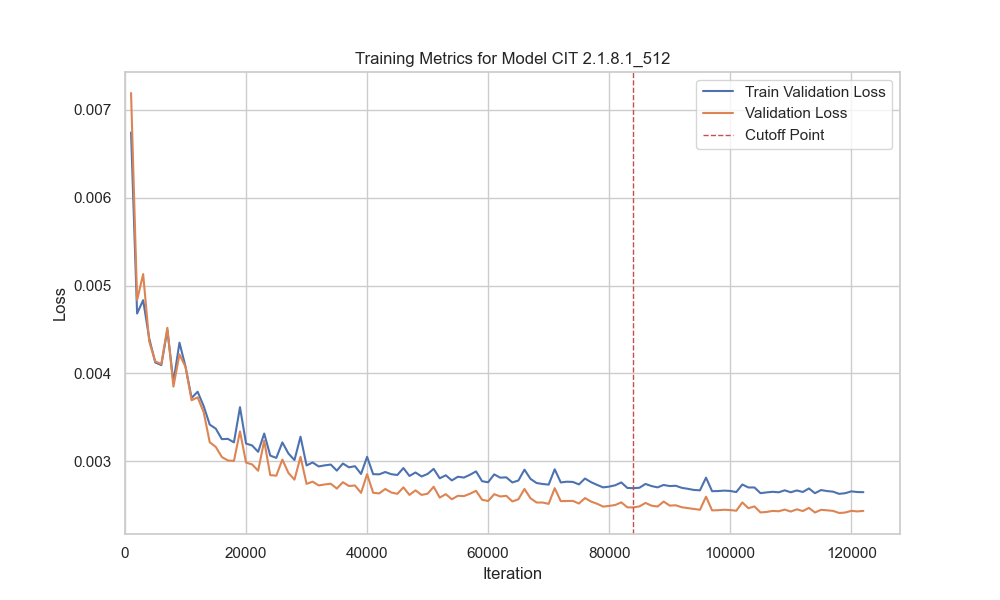
\includegraphics[width=0.9\textwidth]{imgs/Training_Metrics_CIT 2.1.8.1_512.png}
        \caption{Loss plot of the CIT [model 4]}
        \label{fig:Training_Metrics_CIT512}
    \end{figure}

    The figure above displays the training metrics for the Column Image Transformer [model 4] CIT 2.1.8.1\_512, illustrating the loss over iterations during the training phase. The blue line signifies the training validation loss, and the orange line represents the validation loss throughout the training iterations. The graph shows a consistent decline in both metrics, indicating that the model is learning and improving its predictive accuracy over time. The 'Cutoff Point,' indicated by the dashed red line, marks the iteration at which the model is used in the examples presented in this thesis since it has not shown further improvement beyond this point. An unusual behavior observed is that the validation loss is lower than the training validation loss, which is uncommon. This could be the case due to various factors, such as a high dropout rate and needs further investigation.

    \subsubsection{Experimental Results}

    Multiple experiments are conducted to evaluate the performance of the CIT model. These experiments are designed to test the models ability to generate images, the quality of the generated images, and the models performance across different scenarios. The results are analyzed to identify the strengths and weaknesses of the model.
    
    In each test, the end of the seed pixels are marked with a purple line on the left side of the image.
    
    \begin{itemize}
        \item \textbf{Color test:} To assess the models capability to generate specific colors, it is challenged with 11 different images with a width of 32 and a height of 128 pixels. Each test image is composed of a single color filling 128 positions in the models context. The model then generates the next 32 pixels for each image.
    
        \begin{figure}[H]
            \centering
            % First row
            \begin{minipage}{0.45\textwidth}
                \centering
                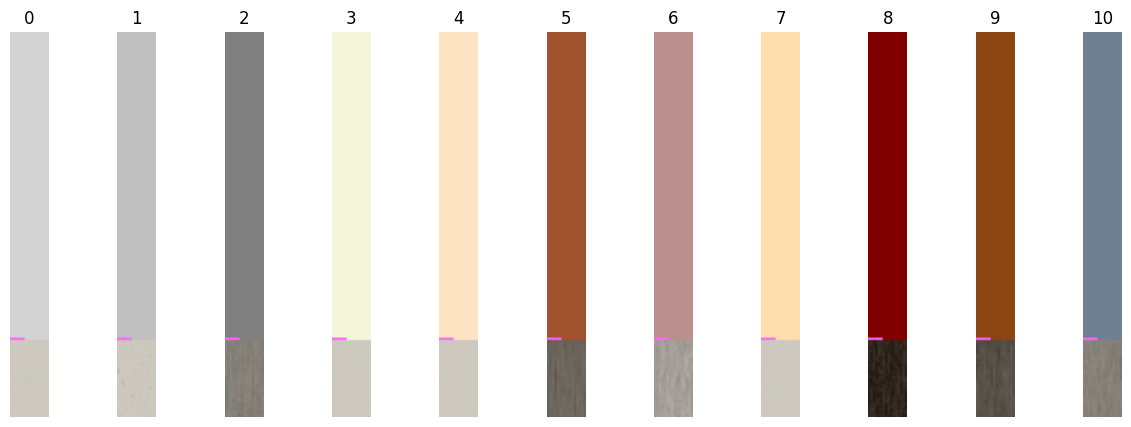
\includegraphics[width=\textwidth]{imgs/ColorTest_2.1.7.1_OldData.png} 
                \subcaption{[model 0] 2.1.7.1}
                \label{fig:test1_M0_Cit}
            \end{minipage}
            \hfill
            \begin{minipage}{0.45\textwidth}
                \centering
                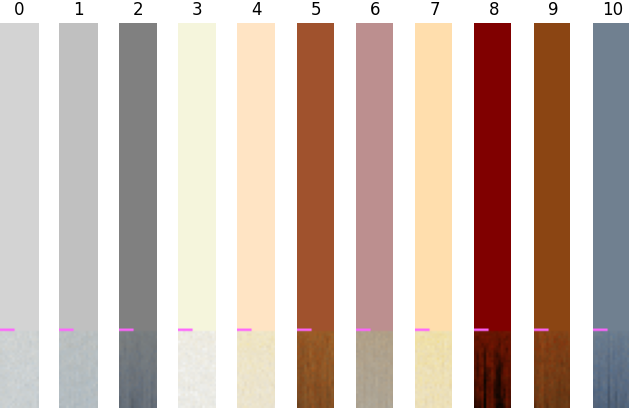
\includegraphics[width=\textwidth]{imgs/ColorTest_2.1.8.1_128.png} 
                \subcaption{[model 1] 2.1.8.1 [128 Context]}
                \label{fig:test1_M1_Cit}
            \end{minipage}
    
            % Second row
            \begin{minipage}{0.45\textwidth}
                \centering
                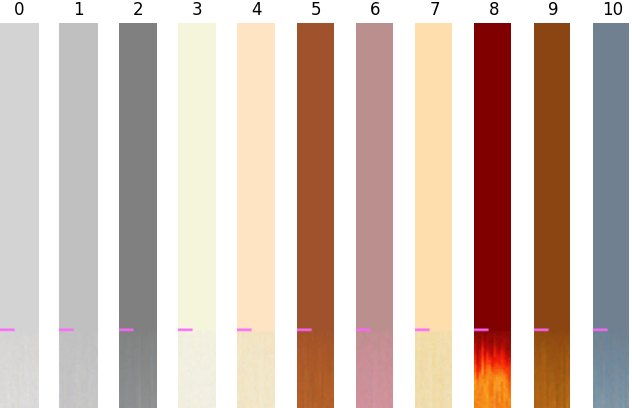
\includegraphics[width=\textwidth]{imgs/ColorTest_2.1.8.1_256.png} 
                \subcaption{[model 2] 2.1.8.1 [256 Context]}
                \label{fig:test1_M2_Cit}
            \end{minipage}
            \hfill
            \begin{minipage}{0.45\textwidth}
                \centering
                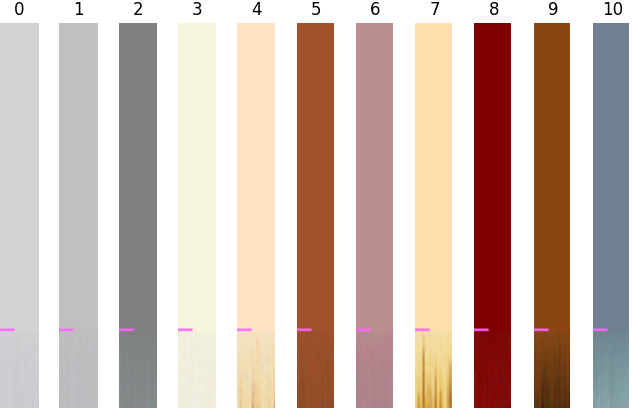
\includegraphics[width=\textwidth]{imgs/ColorTest_2.1.8.1_512.png} 
                \subcaption{[model 4] 2.1.8.1 [512 Context]}
                \label{fig:test1_M3_Cit}
            \end{minipage}
            \caption{Color test with four different models}
        \end{figure}
    
        As shown in the images above, model [0] struggles to generate the correct colors due to the limited size of its old small dataset compared to Models [1-3]. Model [1] generally produces accurate colors but faces difficulties with some. Model [2] generates all colors correctly, but inconsistencies start appearing in column 8. The model may begin changing colors due to its training to recognize patterns such as flowers or carpets in the training data. Model [4] consistently generates the correct colors but begins to create patterns in some columns, potentially indicating that the model is overfitting.
 
        \item \textbf{Zebra pattern test:} The second test assesses whether the model can generate a zebra pattern. The model is provided with both a vertical and a horizontal test image featuring black and white stripes, each stripe being 4 pixels wide. It then generates the next 32 pixels. 

        \begin{figure}[H]
            \centering
            % First row
            \begin{minipage}{0.45\textwidth}
                \centering
                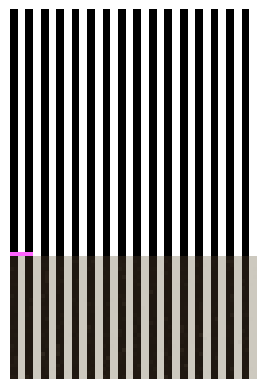
\includegraphics[width=0.5\textwidth]{imgs/ZebraTestV_2.1.7.1_OldData.png} 
                \subcaption{[model 0] 2.1.7.1}
                \label{fig:test2_0_M0_Cit}
            \end{minipage}
            \hfill
            \begin{minipage}{0.45\textwidth}
                \centering
                
\includegraphics[width=0.5\textwidth]{imgs/ZebraTestV_2.1.8.1_512.png} 
                \subcaption{[model 4] 2.1.8.1 [512 Context]}
                \label{fig:test2_0_M5_Cit}
            \end{minipage}
            \caption{Zebra test vertical with two different models}
        \end{figure}

        As shown in the images above, the model with the newer dataset model[4] generates the colors in the zebra pattern more accurately than the model with the older dataset model[0]. Models [0-2] perform similarly. The vertical test is particularly interesting to observe when the column model is altered to see pixels from both the left and the right sides of the current column, assessing whether it can still perfectly continue generating the pattern.


        \begin{figure}[H]
            \centering
            % Second row
            \begin{minipage}{0.45\textwidth}
                \centering
                
\includegraphics[width=0.5\textwidth]{imgs/ZebraTestH_2.1.7.1_OldData.png} 
                \subcaption{[model 1] 2.1.8.1}
                \label{fig:test2_1_M0_Cit}
            \end{minipage}
            \hfill
            \begin{minipage}{0.45\textwidth}
                \centering
                
\includegraphics[width=0.5\textwidth]{imgs/ZebraTestH_2.1.8.1_512.png} 
                \subcaption{[model 4] 2.1.8.1 [512 Context]}
                \label{fig:test2_1_M5_Cit}
            \end{minipage}
            \caption{Zebra test horizontal with two different models}
        \end{figure}

        Unfortunately, the model struggles to generate the zebra pattern horizontally. The model with the newer dataset model [4] more accurately renders the colors in the zebra pattern than the model with the older dataset model [0], but both models struggle to correctly continue the pattern. Model [4] can recognize that the next pixel in the pattern should be dark but quickly loses context. This could be due to the dataset being too small or the model size being insufficient to fully understand the pattern. The images suggest that model [4] is better than model [1] but still fails to generate the pattern correctly.
       
    \end{itemize}

    \subsubsection{Challenges and Limitations}

    The CIT model has some limitations and challenges that require attention. The primary issue is its limited context to only one column, which hampers its ability to generate complex patterns requiring a broader visual spectrum. Additionally, similar to some text-based Transformer models, the CIT model struggles with generating coherent long sequences, often using its recent outputs as a basis for predicting subsequent pixels. This can lead to errors accumulating over time, particularly evident in longer image sequences where the model fails to maintain the specific pattern. 

    To address these limitations, methods used in text-based models, such as scaling up the model size and expanding the training dataset, can be considered. Scaling the model could involve increasing the dimensionality of the embeddings or adding more layers, which might help the model capture more complex dependencies. However, expanding the dataset was not feasible in this thesis due to time constraints and the extensive duration of the dataset collection process.

    Introducing a text prompt feature could significantly enhance the usability and flexibility of the CIT model. This feature would allow users to guide the generation process using descriptive language, making it easier to specify desired outcomes without relying solely on seed pixels. Such a capability would not only improve user interaction but could also potentially help the model deal with complex pattern generation by providing additional contextual information. Exploring this possibility could be a valuable direction for future research.

    \newpage
    

\subsection{Spiral Image Transformer}

    The Spiral Image Transformer, as implied by its name, is a transformer-based model specifically designed to process image data by unrolling pixels in a spiral pattern. This approach stands in contrast to the CIT Model, which processes data using a column-by-column method.

    \begin{figure}[H]
        \centering
        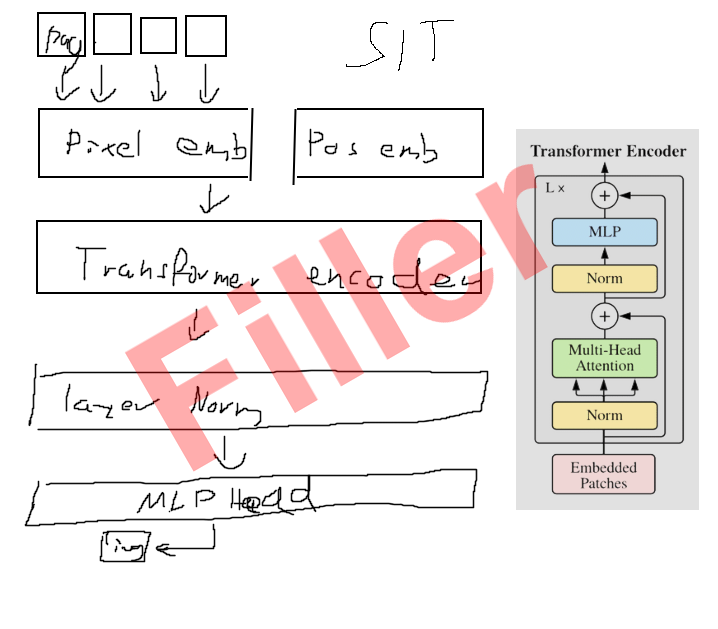
\includegraphics[width=0.8\textwidth]{imgs/SITModel.png}
        \caption{Spiral Image Transformer model structure}
        \label{fig:SpiralImageTransformer}
    \end{figure}

    The visual representation above illustrates the operational steps of the SIT model. Similar to the CIT model, it begins by loading and converting the data. However, it diverges in its method by transforming the data into a spiral format, instead of using the columnar approach. Like its counterpart, this model embeds pixels, from 3 colors to a higher-dimensional embedding space represented by \(N_{\text{EMBD}}\). Positional embeddings are then added. Similar to the CIT model, transformer layers are used to further process the data. The embedded data is finally processed by a (MLP), which converts it back into the original 3-color format. After this step, the spiral-formatted data is restructured into the original image layout.

    \subsubsection{Spiral Data Processing}

    To transform the data, which is loaded by the DataLoader and iterated over, into a spiral format, the width and height dimensions are first squeezed into a single dimension. This resulting tensor has the shape (Batch, Color Channels, Spiral Length). The next step involves indexing the data into the spiral form. For more detailed information on this indexing process, refer to \autoref{fig:spiral_indexing_1}. The restructured tensor is then processed like how the data is handled in the Column Image Transformer model. The following code block illustrates the process used to convert the data into a spiral format.

    \begin{figure}[H]
        \centering
        \begin{lstlisting}[language=Python]
def get_batch(data):
    # Batch_size, Color Channels, Height, Width
    B, C, H, W = data.shape

    spiral_data = torch.zeros_like(data.view(B, C, -1))

    spiral_data[:,:,spiral_indices.flatten()] = data.view(B, C, -1)

    source = spiral_data[:, :, :BLOCK_SIZE]
    label = spiral_data[:, :, 1:BLOCK_SIZE+1]

    source = rearrange(source, 'b c h -> b h c')
    label = rearrange(label, 'b c h -> b h c')

    return source, label
        \end{lstlisting}
        \caption{Python function to get data in a spiral form}
        \label{fig:spiral_indexing_code}
    \end{figure}

    \subsubsection{Spiral generation}
    \label{sec:spiral_generation}
    The conversion of data into a spiral form needs to be highly efficient because the code block will execute for every training step. Therefore, a simple nested for loop is insufficient to rearrange the data into the desired form. In this example, fancy indexing is used to convert the data into a spiral form. Thus, the data tensor is indexed with a flattened two-dimensional tensor containing the indices of the spiral form.

    At the start of the model training script, one indexing spiral is created to be used for all images in the dataset. The following code block illustrates the creation of the spiral index tensor.

\begin{figure}[H]
\centering
\begin{lstlisting}[language=Python]
def create_spiral(n): # n = width and height
    
    matrix = [[0] * n for _ in range(n)] # Initialize n x n matrix

    x, y = 0, 0
    # Direction vectors (right, down, left, up)
    dx = [0, 1, 0, -1]
    dy = [1, 0, -1, 0]
    direction = 0

    for i in range(n * n - 1, -1, -1):  # Start (35 for 6x6)
        matrix[x][y] = i
        nx = x + dx[direction]
        ny = y + dy[direction]

        # Change direction if the next position: out of bounds or filled
        if nx<0 or nx>=n or ny<0 or ny>=n or matrix[nx][ny]!=0:
            direction = (direction + 1) % 4  # Change direction
            nx = x + dx[direction]
            ny = y + dy[direction]

        x, y = nx, ny
    
    return torch.tensor(matrix)
\end{lstlisting}
\caption{Python function to create a spiral index tensor}
\label{fig:spiral_matrix}
\end{figure}

    The code above generates a square matrix of size n by n, then fills it with numbers in a spiral pattern, starting from the outer edge and spiraling inwards clockwise. Each cell of the matrix is assigned a unique number, beginning from the highest value in the top-left corner and decreasing by one with each step along the spiral path until reaching zero at the center or the end of the spiral. The spiral formation is achieved by moving right, then down, then left, then up, and repeating this sequence, adjusting direction whenever the next step would go out of bounds or into a cell that is already been filled.

    The generated spiral index tensor is then used to index the data tensor, effectively converting it into a spiral form. The following image illustrates the process of converting a 7x7 image.
    
    
    \begin{figure}[H]
    \centering
    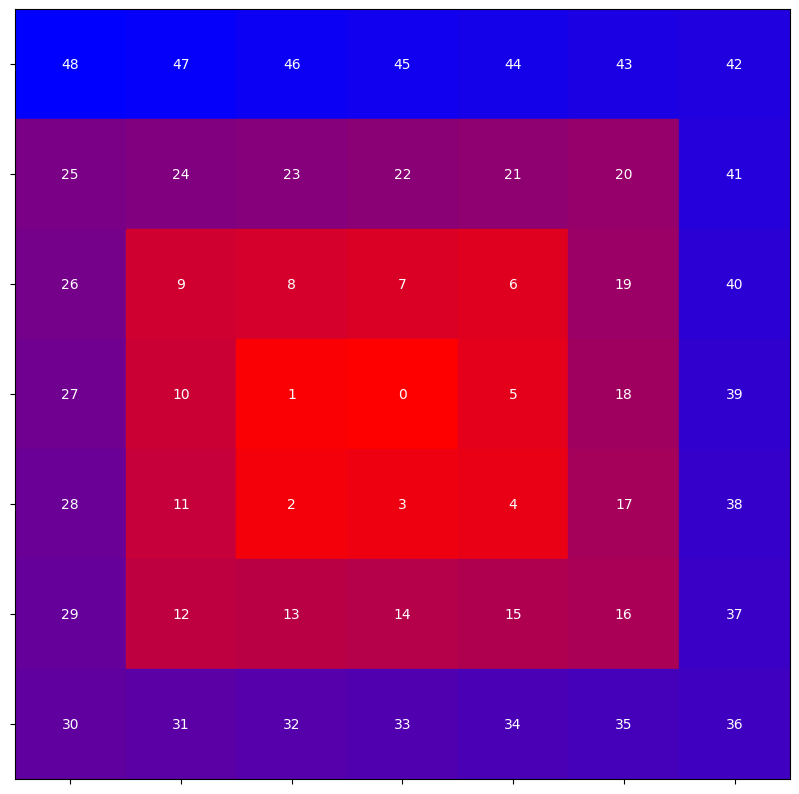
\includegraphics[width=0.6\textwidth]{../code/dataAnalysis/plots/exampleImgs/spiralShowcase1.png}
    \caption{7x7 image with a spiral index overlay}
    \label{fig:spiral_indexing_1}        
    \end{figure}

    \begin{figure}[H]
    \centering
    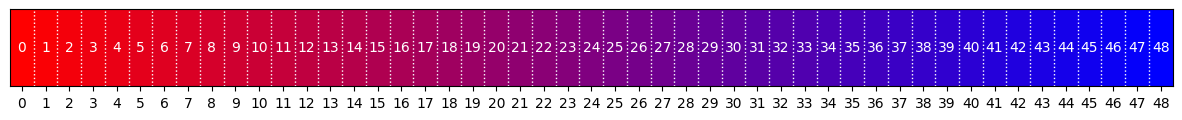
\includegraphics[width=1\textwidth]{../code/dataAnalysis/plots/exampleImgs/spiralShowcase0.png}
    \caption{7x7 Image flattened into the spiral form} 
    \label{fig:spiral_indexing_0}        
    \end{figure}

    As shown in \autoref{fig:spiral_indexing_1}, the pixels of the image are labeled with their respective indices 0, \dots, 48. The image is then unrolled into a single dimension, as shown in \autoref{fig:spiral_indexing_0}. The centering pixel is the first element of the spiral, and the spiral continues counterclockwise from there. In the model script, the dimensions for width and height typically exceed a width of 7, yet the underlying process remains unchanged.



\subsubsection{Model Architecture}

Similar to the CIT model, the addition of positional embeddings is handled in the same manner. This is because the data is transformed into a spiral pattern, allowing the addition of positional embeddings to remain unchanged. Additionally, the transformer layer operates identically. For more information on the transformer layer, see the CIT model \autoref{sec:transformer_CIT}.


\subsubsection{Training the Model}

This model is trained using the Adam optimizer with a learning rate of \(3 \times 10^{-5}\). The loss function used is the Mean Squared Error (MSE) loss. Both training sizes of the model are trained for 4 epochs with a batch size of 8 for the small model and 4 for the big model. The model is trained on the x512 dataset. All the relevant trained SIT models [model 5-6] with their corresponding parameters can be found in detail in the appendix, see \autoref{sec:trained_models_hyperparameters}.

\begin{figure}[H]
    \centering
    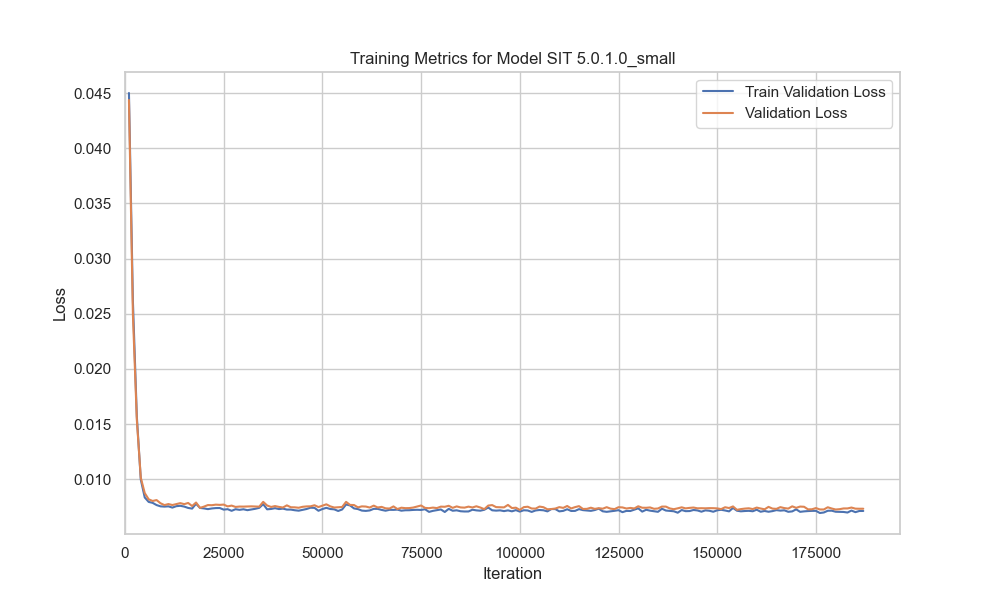
\includegraphics[width=0.9\textwidth]{imgs/Training_Metrics_SIT 5.0.1.0_small.png}
    \caption{Loss plot of the SIT [model 5]}
    \label{fig:Training_Metrics_SITSmall}
\end{figure}

\subsubsection{Experimental Results}

A series of experiments were carried out to assess the capabilities of the Spiral Image Transformer (SIT) model like the CIT Model. The outcomes of these experiments provide insights into the efficacy of the SIT model and highlight potential areas for improvement.

In each of the tests, the end of the seed pixels is marked with a purple pixel indicating the beginning of the generation.

    \begin{itemize}
        \item \textbf{Color test:} To evaluate the color capabilities of the model, a test image with a solid color with a size of 36x36 pixels is provided to the model. The model is then tasked with generating a new image that is 42x42 pixels in width. The test is conducted using two different models, one small and one large.

        \begin{figure}[H]
            \centering
            % First row
            \begin{minipage}{0.48\textwidth}
                \centering
                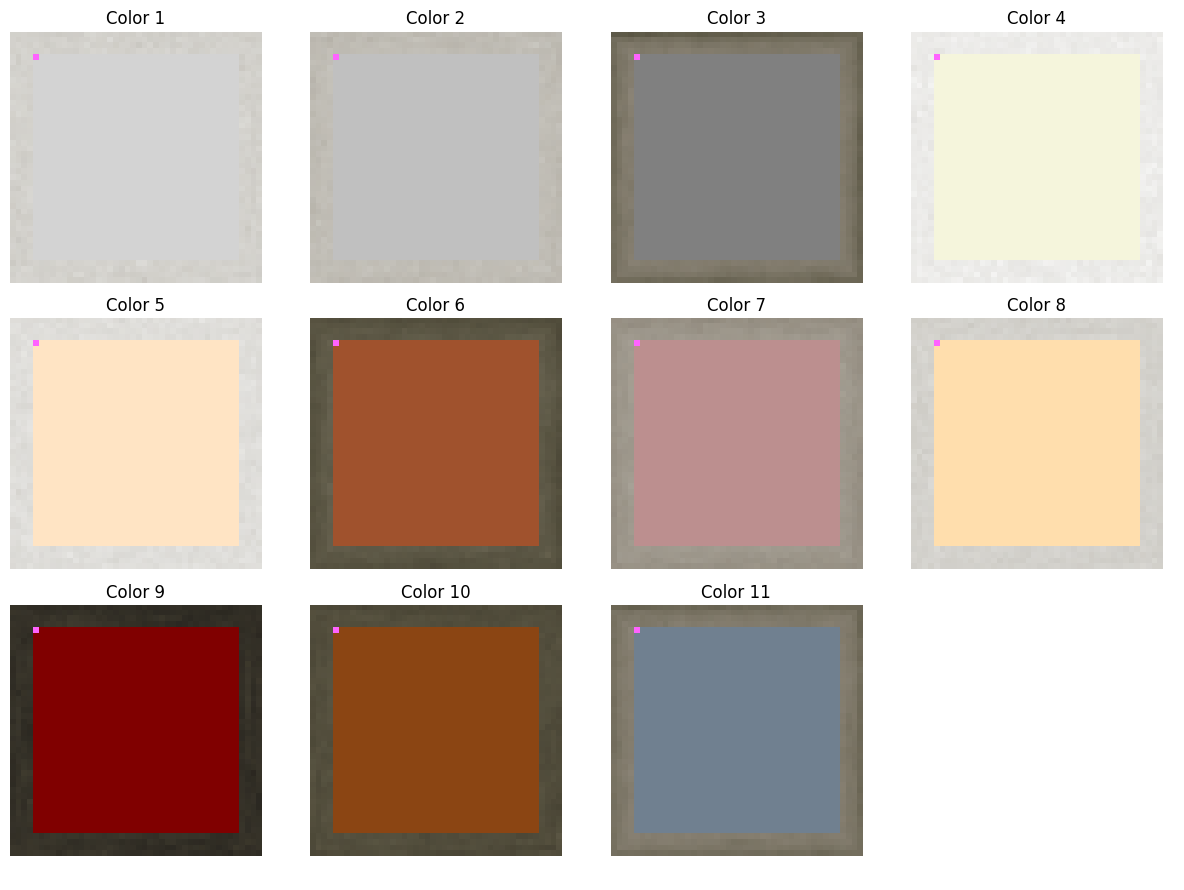
\includegraphics[width=\textwidth]{imgs/ColorTest_5.0.1.0_small.png} 
                \subcaption{[model 5] 5.0.1.0 small}
                \label{fig:test0_1_M4_SIT}
            \end{minipage}
            \hfill
            \begin{minipage}{0.48\textwidth}
                \centering
                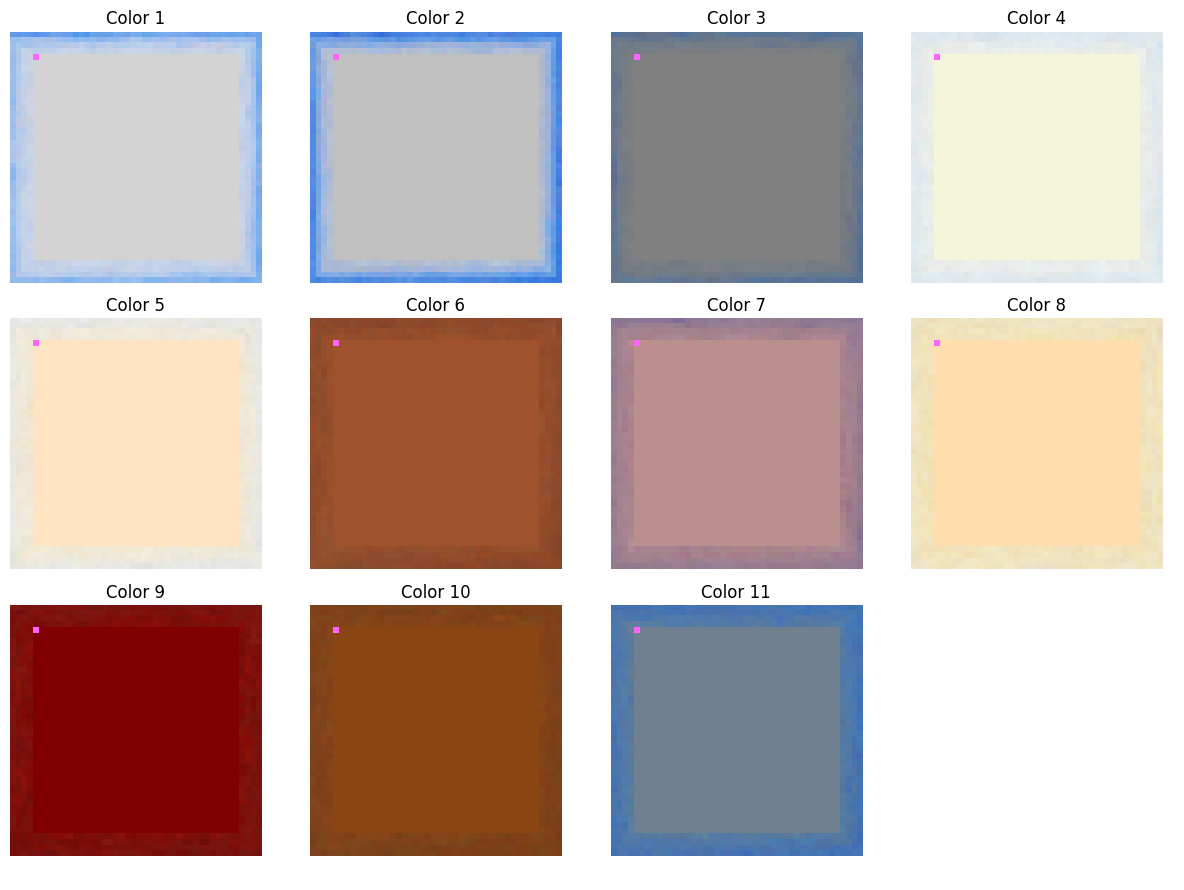
\includegraphics[width=\textwidth]{imgs/ColorTest_5.0.1.0_big.png} 
                \subcaption{[model 6] 5.0.1.0 big}
                \label{fig:test0_2_M5_SIT}
            \end{minipage}
            \caption{Color test with two different model sizes}
        \end{figure}
        
        As depicted in the images above, the smaller model cannot even come close to the desired color output. The larger model performs somewhat better but still struggles to produce the correct color output, especially with the lighter gray shades.
        
        \item \textbf{Image Continuation Test:} The image continuation test is designed to evaluate the model's ability to expand an image. The model is provided with a test image measuring 25 pixels, see \autoref{fig:test2_init_SIT} and is tasked with generating around it to a width of 44 pixels.

        \begin{figure}[H]
            \centering
            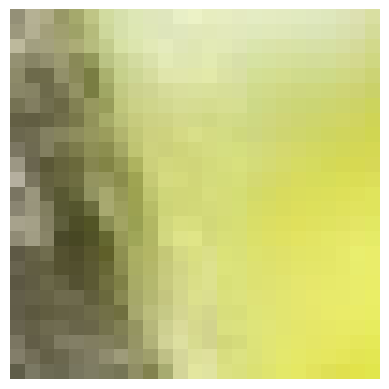
\includegraphics[width=0.3\textwidth]{imgs/ImageTest_5.0.1.0_init.png}
            \caption{Initial test image}
            \label{fig:test2_init_SIT}
        \end{figure}
        
        \begin{figure}[H]
            \centering
            
\includegraphics[width=\textwidth]{imgs/ImageTest_5.0.1.0_flattend.png}
            \caption{Test image flattened into spiral form}
            \label{fig:test2_flattend_SIT}
        \end{figure}
        
        \autoref{fig:test2_flattend_SIT} shows the test image flattened into the spiral form.
        
        \begin{figure}[H]
            \centering
            % First row
            \begin{minipage}{0.48\textwidth}
                \centering
                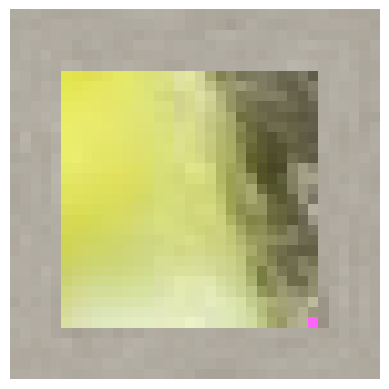
\includegraphics[width=0.8\textwidth]{imgs/ImageTest_5.0.1.0_small.png} 
                \subcaption{[model 5] 5.0.1.0 small}
                \label{fig:test2_1_M4_SIT}
            \end{minipage}
            \hfill
            \begin{minipage}{0.48\textwidth}
                \centering
                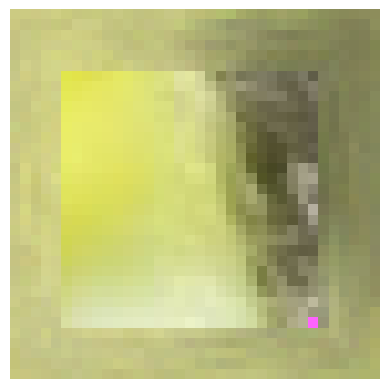
\includegraphics[width=0.8\textwidth]{imgs/ImageTest_5.0.1.0_big.png} 
                \subcaption{[model 6] 5.0.1.0 big}
                \label{fig:test2_2_M5_SIT}
            \end{minipage}
            \caption{Image continuation test with two different model sizes}
            \label{fig:test2_result_SIT}
        \end{figure}
        
        As depicted in \autoref{fig:test2_result_SIT}, the smaller model has difficulty producing the correct color output, focusing primarily on the last gray pixels. In contrast, the larger model performs better, generating a color closer to the desired output. It is important to note that the big model correctly captures that the image should be a light green color on the left side and a gray/dark green color on the right side. This indicates that the model can understand the positional context within the image. However, the model still struggles to generate a clear output.
        

        \item \textbf{Spiral Pattern Test:} The third test evaluates whether the model can accurately generate colors in a rainbow spiral pattern. This test is conducted in a manner very similar to the previous test but provides a more detailed perspective on certain problems. The model starts generating in the upper left corner and continues downwards, then to the right in a counterclockwise motion. The purple pixel indicates the beginning of the generation. The test image is rotated 90 degrees four times to give the model four different starting locations.

        \begin{figure}[H]
            \centering
            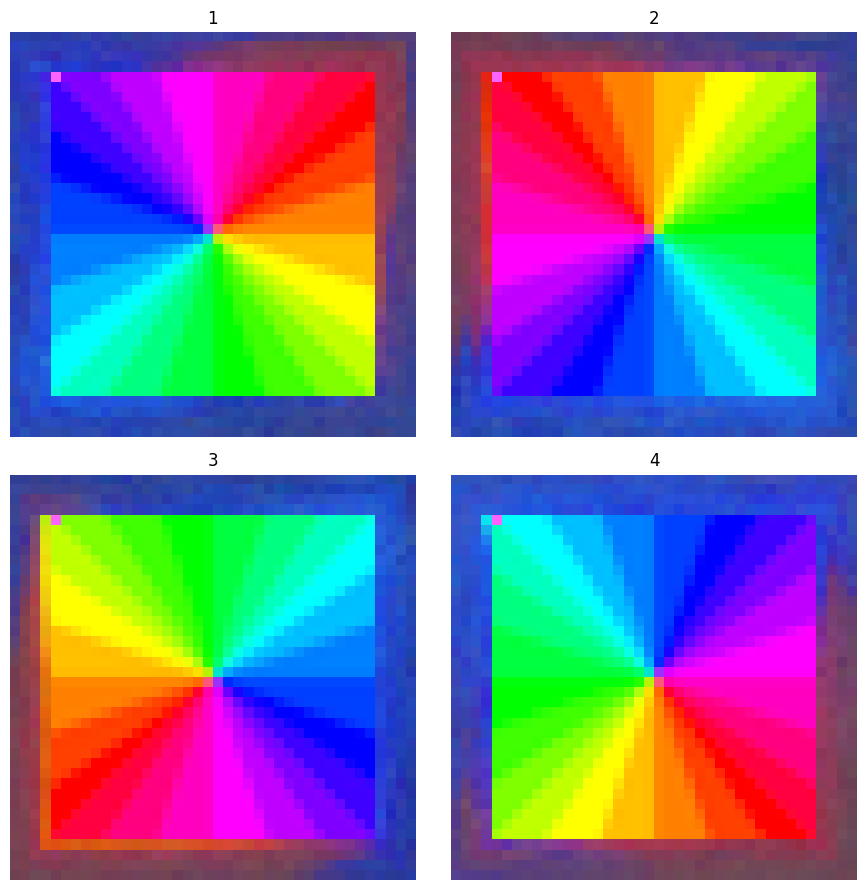
\includegraphics[width=0.7\textwidth]{imgs/RainbowImageTest_5.0.1.0_big.png}
            \caption{Rainbow spiral pattern test SIT [model 6]}
            \label{fig:test3_SIT}
        \end{figure}
        
        As demonstrated in \autoref{fig:test3_SIT}, the model tends to favor the generation of blue or red colors while avoiding yellow, purple, and especially green colors. However, it is noticeable in Image No. 4 that the model generates red accents, although this color is on the opposite side of the starting point. The issues could be due to a lack of training data or the model's size, which needs further investigation.
        

    \end{itemize}

    \subsubsection{Challenges and Limitations}

    As revealed in the experimental section, the Spiral Image Transformer (SIT) model faces difficulties in accurately generating the intended color outputs. This challenge could be anticipated, given that the SIT model's task is inherently more complex than that of the Column Image Transformer (CIT) model. A pattern that progresses one dimensional in a single column is far simpler to learn than one that spirals in two dimensions. The smaller SIT model has an equivalent number of parameters to the smallest CIT model and was trained on an identical dataset, yet its performance is noticeably inferior. Similarly, the larger SIT model holds a parameter count on par with the mid-sized CIT model but falls short in the color tests.

    The limitations experienced by the SIT model could be partially attributed to the insufficiently diverse training dataset. Expanding the dataset, introducing more variance in the training examples, and scaling up the model's complexity could potentially fix its current deficiencies. Moreover, equipping the model with additional contextual data, such as the precise location of a random crop, might improve its capacity for understanding and interpreting the broader context of an image.

    Incorporating a text prompt feature presents could result in a big improvement. By translating descriptive language into visual cues, a text prompt could guide the SIT model toward generating more accurate outputs, potentially reducing or even eliminating the need for seed pixels in some cases.

    Nevertheless, the current iteration of the SIT model is considerably resource-intensive. Its inability to generate multiple pixels parallel translates into lengthy runtimes when operated on consumer-grade GPUs.


    \newpage
    
    \section{Conclusion}\label{conclusion}  
    
This section focuses on the evaluation of the performance of the CIT and the SIT.

\subsection{Evaluation of the models}
    
    As a general conclusion it can be said that the data hints that it is possible to generate quickly new assets trow this approach. Due to the fact that the models are relatively small and the training dataset is not that big the output of the models is 

    \subsubsection{performance}
    One the big question is if it is possible to generated assets for video game. Here we can split it into two parts. The first part is to generate assets beforehand in the development cylce and in the second part is is the model so efficient that it is possible to generate assets in real time on a local machine.

    \subsubsection{quality}


\subsection{Execution locally and on the cloud}
    
    

\subsection{Further research}

    \subsubsection{LLM Scaling Laws}


    \subsection{Stable diffusion/ GANs with convolutional neural network} 
    

    \clearpage
    \setcounter{section}{0}
    \renewcommand*\thesection{\Alph{section}}

    \pagenumbering{roman} 
    \section{Appendix}\label{appendix}
    
\subsection{Dataset Plots in the Lab Color Space}\label{sec:app_labPlots}

\begin{figure}[H]
    \centering
    \foreach \i in {-1,...,18}{
      \begin{subfigure}[t]{0.21\textwidth}
        \centering       
        \ifnum \i=-1
            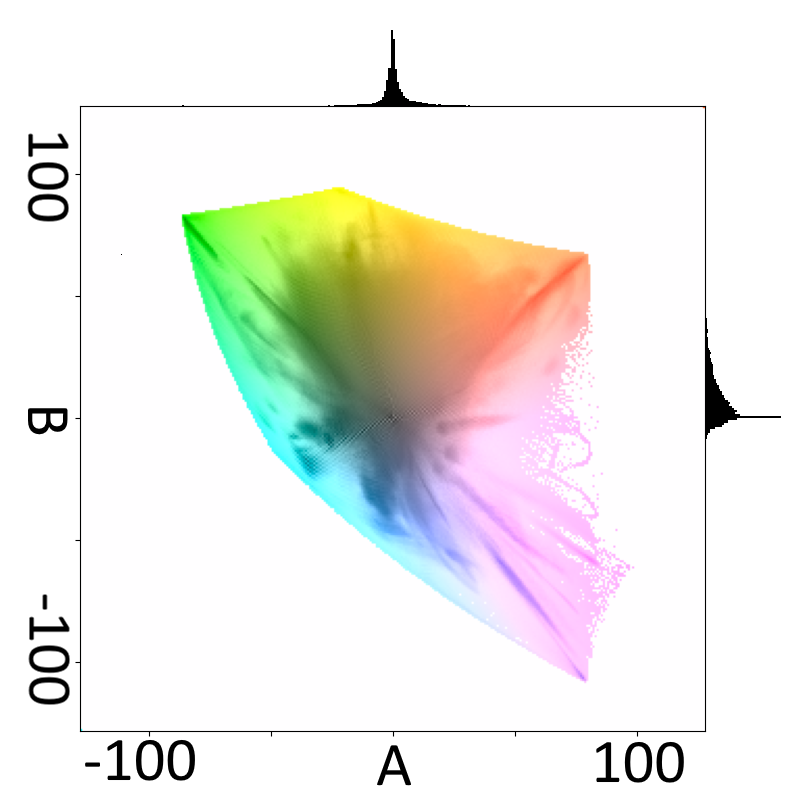
\includegraphics[width=\textwidth]{../code/dataAnalysis/plots/lab/DataCombined_lab.png}
            \caption{All Data}
        \else
            \includegraphics[width=\textwidth]{../code/dataAnalysis/plots/lab/labPlot_\i}
            \caption{source \i}
        \fi

        \label{fig:lab_sub\i}
      \end{subfigure}
      % Use the modulo operation to determine if a line break should be added
      \pgfmathparse{int(mod(\i+2,4))}
      \ifnum\pgfmathresult=0
          \newline
      \else
          \hfill
      \fi
    }
    \begin{subfigure}[t]{0.21\textwidth}
        \centering
        % No image to include, so this is left empty
        \caption*{} % Empty caption
    \end{subfigure}
    \caption*{}
    \addtocounter{figure}{-1}
\end{figure}

\begin{figure}[H]
    \centering
    \foreach \i in {19,...,33}{
      \begin{subfigure}[t]{0.21\textwidth}
        \centering       
        \ifnum \i=-1
            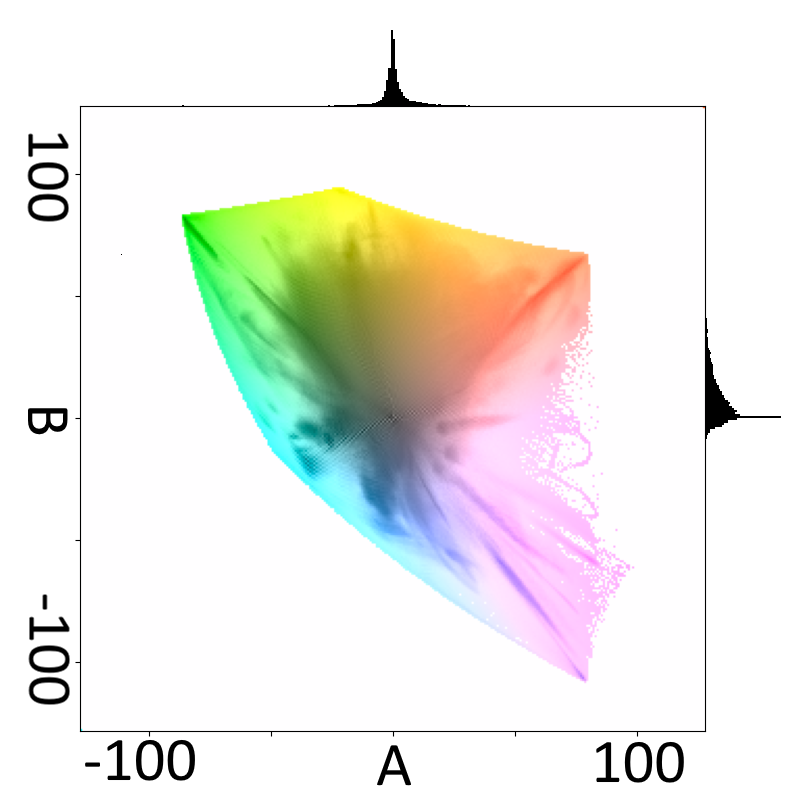
\includegraphics[width=\textwidth]{../code/dataAnalysis/plots/lab/DataCombined_lab.png}
            \caption{All Data}
        \else
            \includegraphics[width=\textwidth]{../code/dataAnalysis/plots/lab/labPlot_\i}
            \caption{source \i}
        \fi

        \label{fig:lab_sub\i}
      \end{subfigure}
      % Use the modulo operation to determine if a line break should be added
      \pgfmathparse{int(mod(\i+2,4))}
      \ifnum\pgfmathresult=0
          \newline
      \else
          \hfill
      \fi
    }
    \begin{subfigure}[t]{0.21\textwidth}
        \centering
        % No image to include, so this is left empty
        \caption*{} % Empty caption
    \end{subfigure}
    \caption{Visualization of datasets plotted in the LAB color space}
    \label{fig:lab_all2}

\end{figure}


\newpage

\subsection{Dataset Plots in the RGB Color Space}

\begin{figure}[H]
    \centering
    \foreach \i in {-1,...,18}{
      \begin{subfigure}[t]{0.21\textwidth}
        \centering

        \ifnum \i=-1
            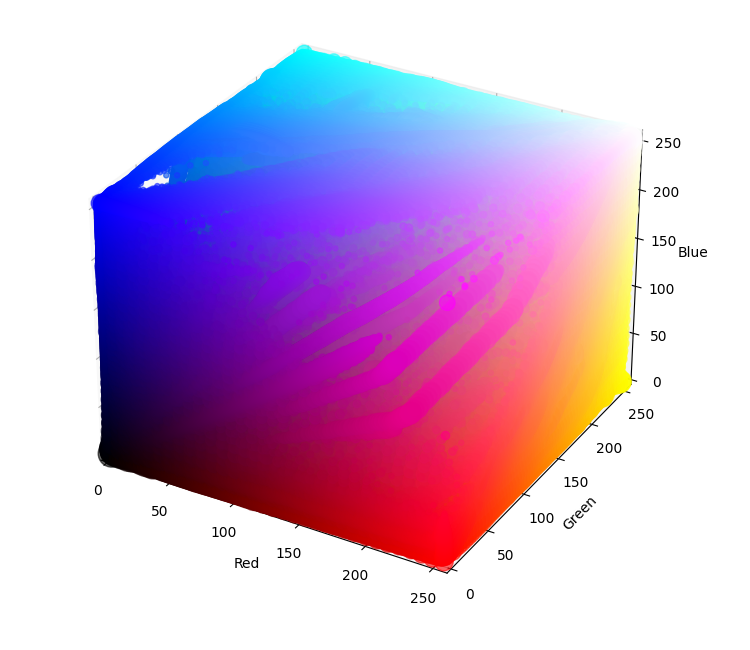
\includegraphics[width=\textwidth]{../code/dataAnalysis/plots/rgb/DataCombined_rgb.png}
        \caption{All Data}
        \else
            \includegraphics[width=\textwidth]{../code/dataAnalysis/plots/rgb/rgbPlot_\i}
            \caption{source \i}
        \fi
        \label{fig:rgb_sub\i}
      \end{subfigure}
      % Use the modulo operation to determine if a line break should be added
      \pgfmathparse{int(mod(\i+2,4))}
      \ifnum\pgfmathresult=0
          \newline
      \else
          \hfill
      \fi
    }
    \begin{subfigure}[t]{0.21\textwidth}
        \centering
        % No image to include, so this is left empty
        \caption*{} % Empty caption
    \end{subfigure}
    \caption*{}
    \addtocounter{figure}{-1}

\end{figure}

\begin{figure}[H]
    \centering
    \foreach \i in {19,...,33}{
      \begin{subfigure}[t]{0.21\textwidth}
        \centering

        \ifnum \i=-1
            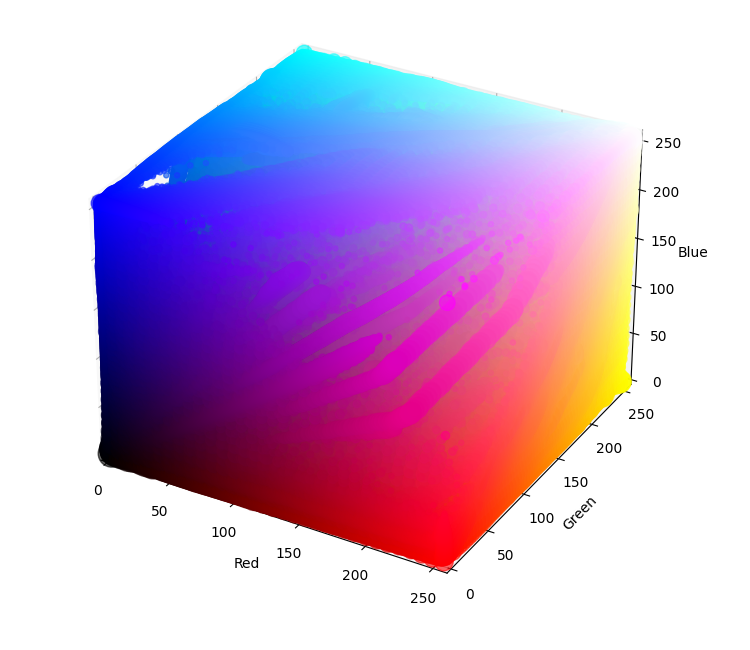
\includegraphics[width=\textwidth]{../code/dataAnalysis/plots/rgb/DataCombined_rgb.png}
        \caption{All Data}
        \else
            \includegraphics[width=\textwidth]{../code/dataAnalysis/plots/rgb/rgbPlot_\i}
            \caption{source \i}
        \fi
        \label{fig:rgb_sub\i}
      \end{subfigure}
      % Use the modulo operation to determine if a line break should be added
      \pgfmathparse{int(mod(\i+2,4))}
      \ifnum\pgfmathresult=0
          \newline
      \else
          \hfill
      \fi
    }
    \begin{subfigure}[t]{0.21\textwidth}
        \centering
        % No image to include, so this is left empty
        \caption*{} % Empty caption
    \end{subfigure}
    \caption{Visualization of datasets plotted in the RGB color space}
    \label{fig:rgb_all}

\end{figure}

\newpage
\begin{landscape}
\subsection{Trained Models with hyperparameters}
\label{sec:trained_models_hyperparameters}


\begin{table}[H]
    \centering
    \begin{threeparttable}
    \caption{Model Configuration Overview}
    \scriptsize
    \begin{tabular}{|c|c|c|c|c|c|c|c|c|c|c|c|c|}
    \toprule
    MODEL & Nr. & VER. & BATCH\_SIZE & BLOCK\_SIZE & N\_EMBD & N\_HEAD & N\_LAYER & PARAMETER\tnote{*} & GPUS & DATASET & VAL\_LOSS\tnote{**}  \\
    \midrule
    \multirow{5}{*}{\rotatebox{90}{CIT}}
    & 0 & 2.1.7.0 & 128 & 128 & 128 & 6 & 6 & 1.22 m & 1 & old Dataset & 0.0082  \\
    & 1 & 2.1.8.0 & 64 & 64 & 128 & 6 & 6 & 1.21 m & 1 & x512 Dataset & 0.0035 \\
    & 2 & 2.1.8.0 Classify & 64 & 64 & 128 & 6 & 6 & 1.25 m & 1 & x512 Dataset & 1.841 \\
    & 3 & 2.1.8.0 & 64 & 256 & 512 & 8 & 8 & 25.66 m & 4 & x512 Dataset & 0.0025 \\
    & 4 & 2.1.8.0 & 32 & 511 & 640 & 9 & 9 & 45.09 m & 4 & x512 Dataset & 0.0024 \\
    \midrule
    \multirow{2}{*}{\rotatebox{90}{SIT}}
    & 5 & 5.0.1.0 & 8 & 4,095 & 128 & 6 & 6 & 1.73 m & 1 & x512 Dataset & 0.0074 \\
    & 6 & 5.0.1.0 & 4 & 4,095 & 512 & 8 & 8 & 27.62 m & 1 & x512 Dataset & 0.0027 \\
    \bottomrule
    \end{tabular}
    \begin{tablenotes}
    \item[*] Figures in millions
    \item[**] Average of the last 5 validation loss values
    \end{tablenotes}
    \end{threeparttable}
\end{table}

\end{landscape}

\newpage

\subsection{Local workstation setup}

\begin{table}[H]
    \centering
    \begin{tabularx}{0.90\textwidth}{|X|X|}
    \hline
    \textbf{Component} & \textbf{Specification} \\ \hline
    Operating System & Microsoft Windows 11 Pro \\ \hline
    CPU & AMD Ryzen 9 7900X 12 cores, 4.7 GHz \\ \hline
    GPU & NVIDIA RTX 3090 \\ \hline
    RAM & 64 GB (DDR5-6000) \\ \hline
    SSD & 2TB Samsung 990 PRO M.2 PCIe 4.0 \\ \hline
    \end{tabularx}
    \caption{Local workstation setup}
    \label{table:workstation_setup}
\end{table}
    
\begin{table}[H]
    \centering
    \begin{tabularx}{0.90\textwidth}{|X|X|}
    \hline
    \textbf{Component} & \textbf{Specification} \\ \hline
    CPU & 2x Intel Xeon "Ice Lake" Platinum 8360Y (36 cores per socket, 2.4 GHz) \\ \hline
    GPU & 4x Nvidia A100 (80GB HBM2, SXM) \\ \hline
    RAM & 1 TB RAM (DDR4-3200) \\ \hline
    SSD & 7.68 TB NVMe local SSD \\ \hline
    \end{tabularx}
    \caption{Single slurm compute node}
    \label{table:server_setup}
\end{table}

\newpage

\subsection{Transformer layer implementation}
\label{sec:transformer_layer_Python}

\begin{lstlisting}[language=Python]
class Head(nn.Module):
""" one head of self-attention """

    def __init__(self, head_size):
        super().__init__()
        self.key = nn.Linear(N_EMBD, head_size, bias=False)
        self.query = nn.Linear(N_EMBD, head_size, bias=False)
        self.value = nn.Linear(N_EMBD, head_size, bias=False)
        self.register_buffer('tril', torch.tril(torch.ones(BLOCK_SIZE, BLOCK_SIZE)))

        self.dropout = nn.Dropout(DROPOUT)

    def forward(self, x):
        # input of size (batch, time-step, channels)
        # output of size (batch, time-step, head size)
        B,T,C = x.shape
        k = self.key(x)   # (B,T,hs)
        q = self.query(x) # (B,T,hs)
        # compute attention scores ("affinities")
        wei = q @ k.transpose(-2,-1) * k.shape[-1]**-0.5 # (B, T, hs) @ (B, hs, T) -> (B, T, T)
        wei = wei.masked_fill(self.tril[:T, :T] == 0, float('-inf')) # (B, T, T)
        wei = F.softmax(wei, dim=-1) # (B, T, T)
        wei = self.dropout(wei)
        # perform the weighted aggregation of the values
        v = self.value(x) # (B,T,hs)
        out = wei @ v # (B, T, T) @ (B, T, hs) -> (B, T, hs)
        return out

class MultiHeadAttention(nn.Module):
""" multiple heads of self-attention in parallel """

    def __init__(self, num_heads, head_size):
        super().__init__()
        self.heads = nn.ModuleList([Head(head_size) for _ in range(num_heads)])
        self.proj = nn.Linear(head_size * num_heads, N_EMBD)
        self.dropout = nn.Dropout(DROPOUT)

    def forward(self, x):
        out = torch.cat([h(x) for h in self.heads], dim=-1)
        out = self.dropout(self.proj(out))
        return out

class FeedFoward(nn.Module):
""" a simple linear layer followed by a non-linearity """

    def __init__(self, n_embd):
        super().__init__()
        self.net = nn.Sequential(
            nn.Linear(n_embd, 4 * n_embd),
            nn.ReLU(),
            nn.Linear(4 * n_embd, n_embd),
            nn.Dropout(DROPOUT),
        )

    def forward(self, x):
        return self.net(x)

class Block(nn.Module):
""" Transformer block: communication followed by computation """

    def __init__(self, n_embd, n_head):
        # n_embd: embedding dimension, n_head: the number of heads we'd like
        super().__init__()
        head_size = n_embd // n_head
        self.sa = MultiHeadAttention(n_head, head_size)
        self.ffwd = FeedFoward(n_embd)
        self.ln1 = nn.LayerNorm(n_embd)
        self.ln2 = nn.LayerNorm(n_embd)

    def forward(self, x):
        x = x + self.sa(self.ln1(x))
        x = x + self.ffwd(self.ln2(x))
        return x
\end{lstlisting}

This code snippet shows the implementation of the transformer layer in the Column Image Transformer and the Spiral Image Transformer. The code above is heavily inspired by the implementation of the script by A.
Karpathy named NanoGPT \autocite{nanoGPTkarpathy2023} \autocite{nanogpt-lecturekarpathy2023}

    \clearpage
    \pagestyle{empty}  
    \pagenumbering{gobble}  
    
    
    \section{Eidesstattliche Erklärung}
    
    Ich versichere, die von mir vorgelegte Arbeit selbständig verfasst zu haben.
    Alle Stellen, die wörtlich oder sinngemäß aus veröffentlichten oder nicht veröffentlichten Arbeiten anderer entnommen sind,
    habe ich als entnommen kenntlich gemacht.\\ 
    Sämtliche Quellen und Hilfsmittel, die ich für die Arbeit benutzt habe, sind
    angegeben. Die Arbeit hat mit gleichem Inhalt bzw. in wesentlichen Teilen noch keiner anderen Prüfungsbehörde vorgelegen.\\\\
    \begin{tabular}{cp{7cm}}
    & \\ 
    & \\ \hline
    \small (Ort, Datum, Unterschrift) & \normalsize \\
    \end{tabular}
    
    
    \newpage
    \printbibliography

    \thispagestyle{empty}
    \newpage

\end{document}

